%% Based on a TeXnicCenter-Template by Tino Weinkauf.

%%\documentclass[12pt,oneside]{report}
\documentclass[twoside,11pt]{article}

\sloppy

%% Language %%%%%%%%%%%%%%%%%%%%%%%%%%%%%%%%%%%%%%%%%%%%%%%%%
%\usepackage[USenglish]{babel} %francais, polish, spanish, ...
\usepackage[T1]{fontenc}
%\usepackage{textcomp}
%\usepackage[ansinew]{inputenc}
%\usepackage{makeidx}	  %% needed to create an index
\usepackage{jsat}
\usepackage{here}
\usepackage{hyperref}   %% sets hyperlinks within a pdf
\usepackage{graphicx}
\usepackage{epstopdf}
\usepackage{parskip}
\usepackage{subcaption}
\usepackage{enumitem}
\usepackage{xcolor}
\usepackage{rotating}
\usepackage{pbox}
\usepackage{listings}
\lstdefinelanguage{smtlib2}
  {alsoletter={-, =},
   morekeywords={set-logic,declare-fun,assert,check-sat,set-info},
   sensitive=false,
   morecomment=[l]{;}}
\lstset{language=smtlib2,
basicstyle=\small\sffamily,
numbers=none,
keywordstyle=\small\bfseries\sffamily,
keywordstyle={[2]\small\bfseries\sffamily\underbar}
}
\usepackage{pifont}
%%\usepackage{lmodern} %Type1-font for non-english texts and characters


%% Packages for Graphics & Figures %%%%%%%%%%%%%%%%%%%%%%%%%%
%\usepackage{graphicx} %%For loading graphic files
%\usepackage{subfig} %%Subfigures inside a figure
%\usepackage{tikz} %%Generate vector graphics from within LaTeX

%\usepackage{mathptmx} %% Times fonts, for math as well

\newcommand{\comment}[2]{\begin{quote}\sc #1\marginpar{\textcolor{red}{$\ast^{\mbox{#2}}$}}\end{quote}}

\newcommand{\tjark}[1]{\comment{#1}{TW}}
\newcommand{\davidd}[1]{\comment{#1}{DD}}
\newcommand{\davidc}[1]{\comment{#1}{DC}}

\newcommand{\rot}[1]{\begin{turn}{90}#1\end{turn}}


\jsatheading{number}{year}{startpage-endpage}
\ShortHeadings{The 2014 SMT Competition}{D.\ Cok et al.}
\firstpageno{1}

\begin{document}

\title{The 2014 SMT Competition}

\author{\name{David R. Cok (chair of organizing committee)}
\email{dcok@grammatech.com} \\
\addr GrammaTech, Inc. \\
\AND
\name{David D\'{e}harbe (co-organizer)}
\email{david@dimap.ufrn.br} \\
\addr Federal University of Rio Grande do Norte, Brazil \\
\AND
\name{Tjark Weber (co-organizer)}
\email{tjark.weber@it.uu.se} \\
\addr Uppsala University, Sweden}

\maketitle

\begin{abstract}
The 2014 SMT Competition was held in conjunction with the SMT Workshop, affiliated with the CAV, IJCAR, and SAT conferences at FLoC 2014, at the Vienna Summer of Logic in July 2014. Eighteen solvers participated from thirteen different research groups, across 34 different logic divisions. The competition was also part of the FLoC Olympic Games event, which gave combined visibility to 14 different competitions related to automated logic problem solving.
The 2014 edition of the SMT Competition was executed for the first time on the StarExec logic solving service. Several records were broken: number of participating solvers, number of new entrants, number of logic divisions, number of benchmarks, and amount of computation. The detailed performance of each solver on each benchmark from this first year using StarExec will be a solid baseline to measure improvements in the state-of-the-art of solver performance in future years.
\end{abstract}

\keywords{SMT solver, SMT-COMP, SMT-LIB, Satisfiability Modulo Theories, competitions}

%\published{December 2014}{revision date}{publication date}

%\davidc{Material to include, from the call: Full articles by competition organizers reporting on SAT-related competitions
  %within FLoC Olympic Games 2014. The articles should describe the competition,
  %its criteria, why it is interesting to the SAT research community, execution
  %environment used, analysis of the results (including how they compare to
  %previous instantiations, if appropriate), and give a summary of the main
  %technical contributions to the field, as well as discussions on lessons
  %learned and suggestions for improvements for future competitions. }


\section{Introduction}
\label{sec:intro}

The SAT decision problem can be generalized by replacing
Boolean variables with atomic predicates built with symbols from a
background theory, or a combination of background theories. The
resulting decision problem is called \emph{Satisfiability Modulo
  Theories}~\cite{DBLP:conf/jelia/Tinelli02}. The background theories of interest arise from
	application domains, such as formal verification or scheduling problems, and include arrays,
bit-vectors, equality with uninterpreted functions, linear and
non-linear arithmetics over integers and real numbers. Also, a theory
may explicitly allow or disallow quantification. Tools addressing the
SMT problem are called \emph{SMT solvers\/}. An SMT solver is often
built by combining a SAT solver with (semi-)decision procedures for
specific theories.

The 2014 SMT Competition (SMT-COMP) continued the series of annual competitions in SMT solver capability and performance that began in 2005. This is the 9th competition in the series, skipping only 2013; in that year an evaluation~\cite{it:2014-017} was performed, rather than a competition.\footnote{The evaluation did not measure solvers against each other, as in a competition. Rather it assessed concerns such as how the design of the competition (e.g., random choice of benchmarks) affects the outcome, the variety and distribution of benchmarks, and the extent to which the competition is dominated by single solvers or by a few solvers or is broadly competitive.}

The competition is held to spur advances in
SMT solver implementations acting on benchmark formulas of practical interest. Public competitions are
a well-known means of stimulating advancement in software tools. For example, in automated
reasoning, the SAT and CASC competitions for propositional and first-order reasoning tools, respectively,
have spurred significant innovation in their fields~\cite{satwebsite,jarvisalo2012international,leberre+03,PSS02}.

The competition is sponsored by the SMT Workshop, which was held in conjunction with the
CAV, IJCAR, and SAT conferences at FLoC 2014~\cite{FLoC2014}, at the Vienna Summer of Logic~\cite{VSL} in July 2014.
Information about the winners
and results of the competition is summarized in this report and is available online at \url{www.smtcomp.org}.  Information
about previous years' competitions is also available at that website and in published summary reports~\cite{springerlink:10.1007/s10817-012-9246-5,DBLP:conf/cade/CokGBD12,it:2014-017}.

In the succeeding sections we describe 
the competition goals (\S\ref{sec:goals}), 
the SMT-LIB language that is the basis for the competition (\S\ref{sec:context}), 
the competition benchmarks (\S\ref{sec:benchmarks}), 
participants (\S\ref{sec:participants}), 
procedure (\S\ref{sec:procedure}),
computational infrastructure (\S\ref{sec:starexec}), 
comparisons with other competitions (\S\ref{sec:OtherCompetitions}), 
the results (\S\ref{sec:results}), 
the place of SMT-COMP in the FLoC Olympic Games (\S\ref{sec:floc}), 
and post-competition activities (\S\ref{sec:post}). 
Section \ref{sec:conclusions} presents observations on this competition and recommendations for the future.

\section{The Competition Goals and Organization}
\label{sec:goals}

In planning the 2014 competition, the organizers' overall goal was to encourage breadth in the capability of SMT solvers.  SMT-COMP 2014 benefited from the evaluation that was performed in 2013 and the experience of previous competitions.  As a result we established the following emphases.  Note that, as described in later sections, the competition is divided into a number of divisions, each focuses on a given logic, and each has its own set of benchmark problems and solvers.
\begin{itemize}
\item In 2012 the competition was narrowed to a smaller number of more significant logics. In response to feedback, in 2014 we reverted to the practice of evaluating solvers in all available divisions.
\item A significant result of the 2013 Evaluation was that the results of previous competitions were highly sensitive to the selection of benchmarks: different random selections of benchmarks resulted in different winning orders in a large fraction of samples. Hence, an aim for 2014 was to use as large a benchmark set as possible in the competition to minimize this effect. We were able to run the competition with all eligible benchmarks. This point is discussed further in~\S\ref{sec:benchmark-selection}.
\item In 2012 some experimental tracks were held: parallel performance, unsat cores, and proof generation. The participation in those tracks was light. Since in 2014 we also had to migrate to using the new StarExec cluster to execute the competition, we held only a main track and an application (incremental) track in the 2014 competition. The organizers still appreciate the value of measuring the performance of solvers on new features such as parallel processing, model generation, unsat core determination, and proof generation, and recommend that these tracks be reinstated in some future edition of the competition.
\item An additional goal was to be able to evaluate the effect of the timeout setting on the competition. Thus a change in 2014 was to increase the timeout limit for a solver processing a given benchmark from 25 minutes (in 2012) to 40 minutes (see \S\ref{sec:procedure} for details on the competition parameters and \S\ref{sec:timeouts} for a discussion on their effects).
\end{itemize}

An important difference between the 2014 competition and previous competitions was that this year's competition was executed on the StarExec cluster, described below in \S\ref{sec:starexec}. All the supporting tools and related procedures needed to be ported to this new framework. With watchful eyes by the organizers and the StarExec team, and with some debugging, the StarExec framework worked well and enabled a larger scale of competition than in previous years.

\section{SMT-LIB Logic, Language and Solvers}
\label{sec:context}

The SMT Competition is a competition among SMT solvers on a set of benchmark logic problems. Each benchmark problem is a combination of definitions and logical assertions expressed with respect to an underlying logical theory and, perhaps, some constraints on the kinds of expressions in that theory. For example,  the logic of linear arithmetic includes the multiplication operation, but only allows multiplication by constants. Each problem is a set of closed formulas over a set of constant or function symbols, possibly including quantification; a solution to the problem is an assignment of each constant and function evaluation to values in a way that satisfies all the problem's assertions. That is, the task is to find a \emph{satisfying assignment} for the benchmark problem or to determine that there is no such assignment. Since the presence of quantified expressions introduces incompleteness, solvers may also produce a potential solution that may be marked as possibly incomplete.

As stated, the goal of SMT-COMP is similar to the goal of the SAT competition. The SMT logic extends SAT by incorporating defined theories, such as the theory of arrays, or of uninterpreted functions, or of arithmetic, or of bit-vectors. In addition, there may be constraints on the set of expressions allowed, such as only linear arithmetic, or only integer difference arithmetic. The theories also define \emph{sorts}, which make the theories a kind of typed first-order logic. Examples of sorts used in current theories are Boolean, Int, Real, bit-vectors of various lengths, and arrays with arbitrary sorts as index and value. Each combination of underlying theories and language constraints is a \emph{logic}.
The names of the logics as used in SMT-LIB are cryptic combinations of initials. For example, AUFLIA is the logic with a
combination of Arrays (A), Uninterpreted Functions (UF), and linear integer arithmetic (LIA). Table \ref{logicAbbreviations} can be used to interpret these names.
\begin{table}
\begin{center}
\begin{tabular}{|l|l|}
\hline
QF\_ & Quantifier-Free \\
A & Arrays \\
UF & Unidentified Functions \\
BV & Bit-Vector \\
L & Linear (arithmetic) \\
N & Non-Linear (arithmetic) \\
IA/RA/IRA & Integer/Real/Mixed arithmetic \\
IDL/RDL & Integer/Real Difference Logic \\
\hline
\end{tabular}
\end{center}
\caption{Abbreviations used in logic names}
\label{logicAbbreviations}
\end{table}

A competition based on benchmark problems needs a standard language in which to express those problems.
For SMT-COMP, that language is the SMT-LIB language (cf.~\url{http://www.smtlib.org}) \cite{BarST-RR-10,BarST-SMT-10,Cok-SMTLIBTutorial-2011}.
In 2010, a significantly reworked version of the language was agreed upon.
This version~2 increased the flexibility and expressiveness of the language while also simplifying the syntax.
It also includes a command language that improves the language's usefulness for interactive applications.
In particular, the standard specifies a typed (sorted), first-order logical language for terms and formulas, a language for specifying background logical theories and logics, and a command language. Some other tools that process SMT-LIB~v2 are listed in the SMT-LIB web pages (cf. \url{http://www.smtlib.org/utilities.shtml}). Further revisions were discussed at the SMT Workshop 2014. One of the goals of the SMT Competition is to encourage use and tool implementations of the SMT-LIB standard.

%However, it is important to note that some tools used in the competition support only a subset of the SMT-LIB command language, leaving out some commands that are essentially syntactic sugar, and are defined as optional in the standard to simplify the burden on competing solvers. This subset is only informally stated and has been stable since 2010. Moreover, the benchmarks only use this subset. This informality did not cause problems in the competition, but it would be preferable to define this subset explicitly. 
%% [DD] Strictly speaking, these commands are optional and a SMT-LIB
%% compliant solver needs not implement them. Which is why I commented
%% out the following sentence 
%%
%% Requiring just a subset for competition works against the goal of
%% producing SMT-LIB-compliant solvers for users.  Fortunately, most
%% mature solvers have implemented nearly all commands of SMT-LIB.
Optional features such as incrementality, proof production, and determining unsat cores are evaluated in specialized tracks, separate from the main competition. The presence of such tracks in the competition has varied from year to year.
  
The following example illustrates part of the language's concrete syntax:

\begin{minipage}{\textwidth}
\begin{quote}
\lstset{frameround=fttt}
\begin{lstlisting}[frame=trBL]
(set-logic UFLIA)
(declare-fun max (Int Int) Int)
(assert (forall ((x Int) (y Int))
   (let ((m (max x y)))
      (and (>= m x) (>= m y) (or (= m x) (= m y))))))
(assert (not (forall ((x Int) (y Int))
   (let ((m (max x y)))
      (= (max (max x y) x) (max x y))))))
(check-sat)
\end{lstlisting}
\end{quote}
\end{minipage}

Commands to the SMT solver are typeset in bold here.  The command
\lstinline{set-logic} sets the background theory: \lstinline{UFLIA} is
the combination of equality with uninterpreted
functions~(\lstinline{UF}) and linear integer
arithmetic~(\lstinline{LIA}). Next, the command
\lstinline{declare-fun} introduces a function symbol, named
\lstinline{max}, which has two arguments of sort \lstinline{Int} and
returns an \lstinline{Int} value. Next, two formulas are asserted. The
first essentially restricts the interpretation of the function named
\lstinline{max} to the standard interpretation. The second expresses
the negation of a property of this operator. The command
\lstinline{check-sat} instructs the SMT solver to check if the
conjunction of the assertions is satisfiable. Here the expected result
is \lstinline{unsat}, indicating that the combination of the two
assertions is unsatisfiable and so, equivalently, the desired property
is valid, given the first assertion.

SMT \textit{solvers} are automated tools that seek a satisfying assignment for a given SMT-LIB problem, or assure that the problem is \emph{unsatisfiable}.
Tools may not be able to solve a given problem, because, for example the tool exhausts available memory or time; a tool is permitted to answer \emph{unknown}. However, giving an incorrect answer (\emph{sat} instead of \emph{unsat}, or vice versa) is considered \emph{unsound} and a serious fault in the tool.


\section{Competition Divisions and Benchmarks}
\label{sec:benchmarks}

The SMT-LIB benchmarks each belong to a specific logic. Each logic is one competition division. For each division, we ran the solvers that entered that division on the benchmarks for that division as one event in the overall competition.

As of June 2014, the SMT-LIB repository contained over 130,000
main-track benchmarks divided into 34 background theories, and
close to 10,000 incremental benchmarks distributed across 8 background
theories. The size of a benchmark file may vary from a few hundred
bytes to several gigabytes. Fig.~\ref{fig:smtlib-bysize} shows the
distribution of the benchmarks by file size.

\begin{figure}
\begin{center}
\begin{tabular}{cc}
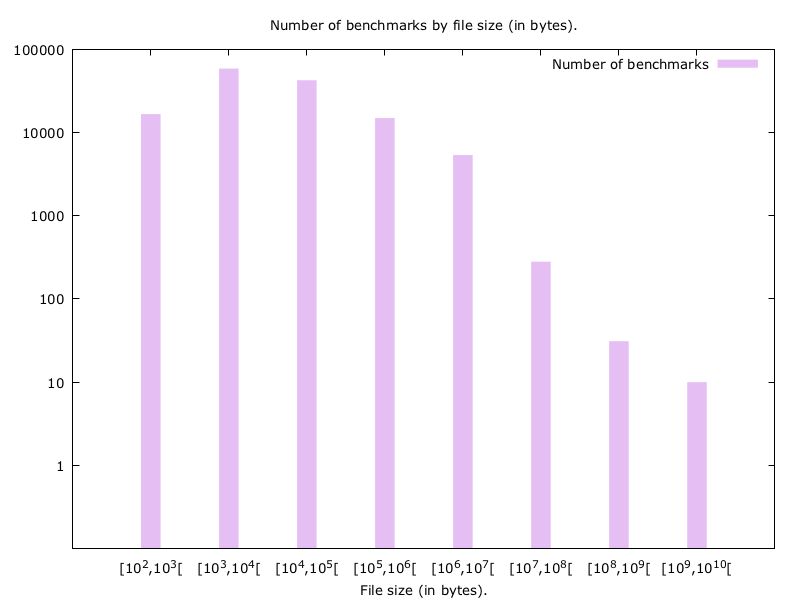
\includegraphics[width=.47\textwidth]{smtlib2-file-count-by-size.png}
&
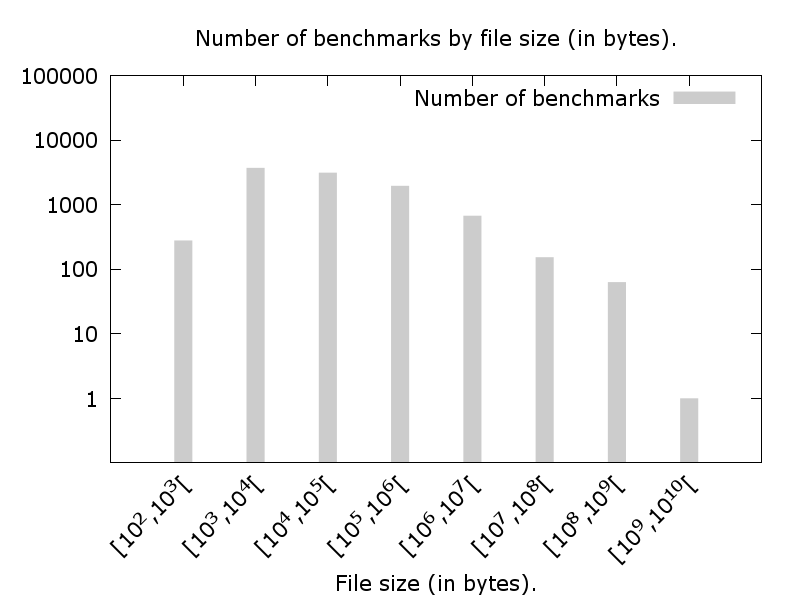
\includegraphics[width=.47\textwidth]{smtlib2-app-file-count-by-size.png}
\\
\\
Non-incremental benchmarks & Application benchmarks
\end{tabular}
\end{center}
\caption{Distribution of SMT-LIB benchmarks by file size.
\label{fig:smtlib-bysize}}
\end{figure}


A sizeable number of benchmarks, on the order of 30,000, were added during the lead up to the competition. Some of these were submitted in previous years but never assessed and uploaded. Many others were supplied by solver developers (including some competitors). All of them went through an iterative curation process to be sure that they were syntactically valid, appropriate metadata was included, and a correct result was established. (Not all of these submissions were through the competition organizers.)

The SMT-LIB coordinators performed a curation step on the entire benchmark library prior to the competition, determining the actual logic to which a benchmark belonged, rather than the super-logic to which it had previously been assigned. This resulted in an expansion of logics with benchmarks from 23 to 34, and also created a number of divisions with only a very few benchmarks. Two divisions were not held because they had no eligible benchmarks.

The 34 logics are shown in Table \ref{Table:benchmarks}. The rightmost column shows the number of benchmarks for that logic in the SMT-LIB collection. Two considerations may make a benchmark ineligible for a competition. First, the benchmark may not have a known result. For newly submitted benchmarks
we made an attempt to determine the correct result of the benchmark; the SMT-LIB coordinators require that two
different solvers solve the benchmark and report the same result. However, for benchmarks with unknown results already in the collection we did not have time to determine their results. We did do this analysis after the competition was over (see~\S\ref{sec:post}).

The second consideration is that the benchmark must be \emph{non-trivial}; a benchmark is deemed trivial if all solvers managed to solve it in less than five seconds during SMT-EVAL 2013.

The numbers of unknown, trivial, and remaining eligible benchmarks are shown in Table \ref{Table:benchmarks}. Note that these numbers vary widely from division to division.


\begin{table}
\caption{Numbers of main-track benchmarks. The second column shows the number of competitive solvers and, in square brackets, the number of demonstration-only solvers. Entries marked * exclude some benchmarks containing partial functions.}
\label{Table:benchmarks}
\centering
\begin{tabular}{|l|r|r|r|r|r|}
\hline
       & \multicolumn{1}{|c|}{\# of} & \multicolumn{4}{|c|}{\# of benchmarks} \\
 Logic & solvers & eligible & unknown  & trivial & total  \\
\hline
ALIA & 3+[1] & 29 & 0 & 13 & 42 \\
AUFLIA & 3+[1] & 4 & 0 & 0 & 4\\
AUFLIRA & 3+[1] & 10791 & 168 & 9055 & 20014 \\
AUFNIRA & 2+[2] & 564 & 468 & 463 & 1495 \\
BV & 2+[1] & 0 & 191 & 0 & 191 \\
LIA & 3+[1] & 46 & 0 & 0 & 46 \\
LRA & 3+[1] & 171 & 450 & 0 & 621\\
NIA & 2+[1] & 9 & 0 & 0 & 9\\
NRA & 2+[1] & 3747 & 66 & 0 & 3813 \\
QF\_ABV & 7+[2] & 6457* & 4191 & 4423 & 15091 \\
QF\_ALIA & 3+[2] & 97 & 0 & 29 & 126 \\
QF\_AUFBV & 2+[2] & 37 & 0 & 0 & 37 \\
QF\_AUFLIA & 4+[2] & 610 & 0 & 399 & 1009\\
QF\_AX & 3+[2] & 335 & 0 & 216 & 551 \\
QF\_BV & 8+[3] & 2488* & 28138 & 546 & 32500 \\
QF\_IDL & 3+[1] & 1315 & 537 & 337 & 2189 \\
QF\_LIA & 4+[3] & 4381 & 1279 & 481 & 6141 \\
QF\_LRA & 4+[2] & 1343 & 208 & 131 & 1682\\
QF\_NIA & 3+[1] & 8327 & 927 & 105 & 9359 \\
QF\_NRA & 3+[1] & 10121 & 1392 & 27 & 11540 \\
QF\_RDL & 3+[1] & 132 & 85 & 38 & 255 \\
QF\_UF & 5+[2] & 4124 & 4 & 2522 & 6650 \\
QF\_UFBV & 2+[2] & 31 & 0 & 0 & 31 \\
QF\_UFIDL & 3+[1] & 311 & 0 & 130 & 441\\
QF\_UFLIA & 4+[2] & 484 & 0 & 114 & 598 \\
QF\_UFLRA & 4+[2] & 1176 & 87 & 367 & 1630 \\
QF\_UFNIA & 2+[1] & 7 & 0 &0 & 7 \\
QF\_UFNRA & 2+[1] & 32 & 11 & 0 & 43\\
UF & 3+[1] & 2830 & 2911 & 7 & 5748 \\
UFBV & 2+[1] & 0 & 191 & 0 & 191 \\
UFIDL & 2+[1] & 49 & 12 & 19 & 80 \\
UFLIA & 3+[1] & 5766 & 5499 & 873 & 12138 \\
UFLRA & 3+[1] & 25 & 0 & 0 & 25\\
UFNIA & 2+[1] & 1587 & 1052 & 712 & 3351 \\
\hline
Total & 18+[3] & 67426 & 47867 & 21007 & 137648 \\
\hline
\end{tabular}
\end{table}

Solvers could participate in any or all divisions at their team's discretion. Most solvers are designed for just one selected logic, but others are intended to be as broadly applicable as their developers have had time to implement. Table~\ref{Table:logics} shows the participation of solvers in various divisions.

\begin{sidewaystable}
\caption{Solver participation in logic divisions}
\label{Table:logics}
\centering
\renewcommand{\mark}[0]{\ding{51}}
%%\small
\setlength\tabcolsep{3pt}
%%\begin{tabular}{|l|c|c|c|c|c|c|c|c|c|c|c|c|c|c|c|c|c|c|c|c|c|c|c|c|c|c|c|c|c|c|c|c|c|c|}
\begin{tabular}{|l|ccccc|cccc|cccccc|cccccc|ccccccc|cccccc|}
\hline
Solver & 	\rot{ALIA} & 	\rot{AUFLIA} & 	\rot{AUFLIRA} & 	\rot{AUFNIRA} & 	\rot{BV} & 	\rot{LIA} & 	\rot{LRA} & 	\rot{NIA} & 	\rot{NRA} & 	\rot{QF\_ABV} & 	\rot{QF\_ALIA} & 	\rot{QF\_AUFBV} & 	\rot{QF\_AUFLIA} & 	\rot{QF\_AX} & 	\rot{QF\_BV} & 	\rot{QF\_IDL} & 	\rot{QF\_LIA} & 	\rot{QF\_LRA} & 	\rot{QF\_NIA} & 	\rot{QF\_NRA} & 	\rot{QF\_RDL} & 	\rot{QF\_UF} & 	\rot{QF\_UFBV} & 	\rot{QF\_UFIDL} & 	\rot{QF\_UFLIA} & 	\rot{QF\_UFLRA} & 	\rot{QF\_UFNIA} & 	\rot{QF\_UFNRA} & 	\rot{UF} & 	\rot{UFBV} & 	\rot{UFIDL} & 	\rot{UFLIA} & 	\rot{UFLRA} & 	\rot{UFNIA} \\
\hline
4Simp & 	 & 	 & 	 & 	 & 	 & 	 & 	 & 	 & 	 & 	 & 	 & 	 & 	 & 	 & 	\mark & 	 & 	 & 	 & 	 & 	 & 	 & 	 & 	 & 	 & 	 & 	 & 	 & 	 & 	 & 	 & 	 & 	 & 	 & 	 \\
Abziz & 	 & 	 & 	 & 	 & 	 & 	 & 	 & 	 & 	 & 	 & 	 & 	 & 	 & 	 & 	\mark & 	 & 	 & 	 & 	 & 	 & 	 & 	 & 	 & 	 & 	 & 	 & 	 & 	 & 	 & 	 & 	 & 	 & 	 & 	 \\
Abziz2 & 	 & 	 & 	 & 	 & 	 & 	 & 	 & 	 & 	 & 	 & 	 & 	 & 	 & 	 & 	\mark & 	 & 	 & 	 & 	 & 	 & 	 & 	 & 	 & 	 & 	 & 	 & 	 & 	 & 	 & 	 & 	 & 	 & 	 & 	 \\
AProVE & 	 & 	 & 	 & 	 & 	 & 	 & 	 & 	 & 	 & 	 & 	 & 	 & 	 & 	 & 	 & 	 & 	 & 	 & 	\mark & 	 & 	 & 	 & 	 & 	 & 	 & 	 & 	 & 	 & 	 & 	 & 	 & 	 & 	 & 	 \\
Boolector & 	 & 	 & 	 & 	 & 	 & 	 & 	 & 	 & 	 & 	 & 	 & 	 & 	 & 	 & 	\mark & 	 & 	 & 	 & 	 & 	 & 	 & 	 & 	 & 	 & 	 & 	 & 	 & 	 & 	 & 	 & 	 & 	 & 	 & 	 \\
Boolector-d & 	 & 	 & 	 & 	 & 	 & 	 & 	 & 	 & 	 & 	\mark & 	 & 	 & 	 & 	 & 	 & 	 & 	 & 	 & 	 & 	 & 	 & 	 & 	 & 	 & 	 & 	 & 	 & 	 & 	 & 	 & 	 & 	 & 	 & 	 \\
Boolector-j & 	 & 	 & 	 & 	 & 	 & 	 & 	 & 	 & 	 & 	\mark & 	 & 	 & 	 & 	 & 	 & 	 & 	 & 	 & 	 & 	 & 	 & 	 & 	 & 	 & 	 & 	 & 	 & 	 & 	 & 	 & 	 & 	 & 	 & 	 \\
CVC3 & 	\mark & 	\mark & 	\mark & 	\mark & 	\mark & 	\mark & 	\mark & 	\mark & 	\mark & 	 & 	 & 	 & 	 & 	 & 	 & 	 & 	 & 	 & 	\mark & 	\mark & 	 & 	 & 	 & 	 & 	 & 	 & 	\mark & 	\mark & 	\mark & 	\mark & 	\mark & 	\mark & 	\mark & 	\mark \\
CVC4 & 	\mark & 	\mark & 	\mark & 	\mark & 	\mark & 	\mark & 	\mark & 	\mark & 	\mark & 	\mark & 	\mark & 	\mark & 	\mark & 	\mark & 	\mark & 	\mark & 	\mark & 	\mark & 	\mark & 	\mark & 	\mark & 	\mark & 	\mark & 	\mark & 	\mark & 	\mark & 	\mark & 	\mark & 	\mark & 	\mark & 	\mark & 	\mark & 	\mark & 	\mark \\
Kleaver-STP & 	 & 	 & 	 & 	 & 	 & 	 & 	 & 	 & 	 & 	\mark & 	 & 	 & 	 & 	 & 	 & 	 & 	 & 	 & 	 & 	 & 	 & 	 & 	 & 	 & 	 & 	 & 	 & 	 & 	 & 	 & 	 & 	 & 	 & 	 \\
Kleaver-portfolio & 	 & 	 & 	 & 	 & 	 & 	 & 	 & 	 & 	 & 	\mark & 	 & 	 & 	 & 	 & 	 & 	 & 	 & 	 & 	 & 	 & 	 & 	 & 	 & 	 & 	 & 	 & 	 & 	 & 	 & 	 & 	 & 	 & 	 & 	 \\
OpenSMT2 & 	 & 	 & 	 & 	 & 	 & 	 & 	 & 	 & 	 & 	 & 	 & 	 & 	 & 	 & 	 & 	 & 	 & 	 & 	 & 	 & 	 & 	\mark & 	 & 	 & 	 & 	 & 	 & 	 & 	 & 	 & 	 & 	 & 	 & 	 \\
raSAT & 	 & 	 & 	 & 	 & 	 & 	 & 	 & 	 & 	 & 	 & 	 & 	 & 	 & 	 & 	 & 	 & 	 & 	 & 	 & 	\mark & 	 & 	 & 	 & 	 & 	 & 	 & 	 & 	 & 	 & 	 & 	 & 	 & 	 & 	 \\
SMTInterpol & 	 & 	 & 	 & 	 & 	 & 	 & 	 & 	 & 	 & 	 & 	\mark & 	&	\mark & 	\mark & 	 & 	 & 	\mark & 	\mark & 	 & 	 & 	 & 	\mark & 	 & 	 & 	\mark & 	\mark & 	 & 	 & 	 & 	 & 	 & 	 & 	 & 	 \\
SONOLAR & 	 & 	 & 	 & 	 & 	 & 	 & 	 & 	 & 	 & 	\mark & 	 & 	 & 	 & 	 & 	\mark & 	 & 	 & 	 & 	 & 	 & 	 & 	 & 	 & 	 & 	 & 	 & 	 & 	 & 	 & 	 & 	 & 	 & 	 & 	 \\
STP-Crypto... & 	 & 	 & 	 & 	 & 	 & 	 & 	 & 	 & 	 & 	 & 	 & 	 & 	 & 	 & 	\mark & 	 & 	 & 	 & 	 & 	 & 	 & 	 & 	 & 	 & 	 & 	 & 	 & 	 & 	 & 	 & 	 & 	 & 	 & 	 \\
veriT & 	\mark & 	\mark & 	\mark & 	 & 	 & 	\mark & 	\mark & 	 & 	 & 	 & 	 & 	 & 	\mark & 	& &		\mark & 	\mark & 	\mark & 	 & 	 & 	\mark & 	\mark & 	&	\mark & 	\mark & 	\mark & 	 & 	 & 	\mark & 	 & 	 & 	\mark & 	\mark &   \\
Yices2 & 	 & 	 & 	 & 	 & 	 & 	 & 	 & 	 & 	 & 	\mark & 	\mark & 	\mark & 	\mark & 	\mark & 	\mark & 	\mark & 	\mark & 	\mark & 	 & 	 & 	\mark & 	\mark & 	\mark & 	\mark & 	\mark & 	\mark & 	 & 	 & 	 & 	 & 	 & 	 & 	 & 	 \\
\hline
{[}MathSAT5] & 	 & 	 & 	 & 	 & 	 & 	 & 	 & 	 & 	 & 	\mark & 	\mark & 	\mark & 	\mark & 	\mark & 	\mark & 	 & 	\mark & 	\mark & 	 & 	 & 	 & 	\mark & 	\mark & 	 & 	\mark & 	\mark & 	 & 	 & 	 & 	 & 	 & 	 & 	 & 	 \\
{[}Z3] & 	\mark & 	\mark & 	\mark & 	\mark & 	\mark & 	\mark & 	\mark & 	\mark & 	\mark & 	\mark & 	\mark & 	\mark & 	\mark & 	\mark & 	\mark & 	\mark & 	\mark & 	\mark & 	\mark & 	\mark & 	\mark & 	\mark & 	\mark & 	\mark & 	\mark & 	\mark & 	\mark & 	\mark & 	\mark & 	\mark & 	\mark & 	\mark & 	\mark & 	\mark \\
{[}CVC4-with-bugfix] &  &  &  & \mark &  &  &  &  &  &  &  &  &  &  & \mark &  & \mark &  &  &  &  &  &  &  &  &  &  &  &  &  &  &  &  &  \\
\hline
\end{tabular}
\end{sidewaystable}

\subsection{Application benchmarks.} 

The language includes commands that allow a fine-grained interaction
with the solver, whereby client tools may incrementally push and pop
symbol declarations and assertions while running various
satisfiability checks, inspecting models, or obtaining unsatisfiability
proofs. Benchmarks problems that have more than one
\lstinline{check-sat} command are called \emph{application} or \emph{incremental
  benchmarks}. Not all SMT solvers support all of these interaction
facilities, and the main track of the competition does not use such
application benchmarks.


\subsection{Selection of benchmarks. \label{sec:benchmark-selection}} 

Due to the mismatch between the amount of available compute time and the number of jobs to run, benchmark selection has been an historical issue for SMT-COMP. In addition to whether a benchmark has a known result or is trivial, the SMT-COMP organizers chose two other factors that affect the selection of benchmarks for SMT-COMP: the benchmark's difficulty and the desire for a distribution of problems. In 2014, the amount of available CPU time was enough to process all benchmarks on all solvers within the timeout defined in the rules. However this could not be anticipated, and the issues described hereafter may happen again, e.g., in case the number or difficulty of benchmarks, number of solvers, or the timeout increase significantly, or the organizers wish to compress the time-frame in which the competition is executed.

Each benchmark is assigned a \emph{difficulty rating}; in 2014, we used the time taken to solve the benchmark by the best performing solver in the 2013 SMT Evaluation. These values were publicly available prior to the competition. The difficulty ratings are used to divide the benchmarks into 5 quintiles. The rules describe a procedure for randomly selecting $N$ out of the eligible benchmarks for a division, with the intent of selecting roughly equal numbers, if they are available, from each of the quintiles.  The seed for the random number generator used for selection is obtained by summing a number supplied by each solver team and the integer portion of the New York Stock Exchange Composite Index at its opening on the day the competition begins.

Benchmarks are also labeled by \emph{category}: simple checks, randomly generated problems from some template (e.g., N-queens problems for various values of N), problems crafted to test a certain capability, and problems obtained from industrial applications. The selection rules favor industrial benchmarks.

Another selection criterion, though not used historically, is to balance the numbers of \textit{sat} and \textit{unsat} benchmarks.

In addition, some kinds of problems may be over-represented in the benchmarks. This may be the case particularly because benchmarks may be submitted by solver developers; a team might add a large number of benchmarks that would then over-represent problems that a particular solver is known to handle well. The rules allow the organizers to limit the selections from sub-populations.

In the end, in 2014, there was sufficient time to use all eligible benchmarks and no further selection was performed. The 2014 organizers did not have the data to make a principled decision on over-representation of particular problem types and so did not select on this basis either. The absence of such selection may have affected the competition results and future organizing teams should reconsider this aspect even if there are sufficient computational resources to execute all benchmarks. The data from SMT-COMP 2014 could be used to inform this decision.



\section{Participants}
\label{sec:participants}

The competition registration requires participants to submit information about each competing solver. In addition, some solver groups provided summaries of their solvers and their recent technical advances.
 Note that although one person is listed as the ``submitter,'' there is generally a team of contributors behind each tool. Some teams submitted more than one tool. The 2014 participants were the following:
\begin{itemize}
\item 4Simp -- submitted by Trevor Hansen (U. Melbourne)
\item AbzizPortfolio -- two versions -- submitted by Mohammed Adbul Aziz (U. Cairo). This solver is atypical in that it is a portfolio solver: based on automated learning over benchmark characteristics, it chooses among other solvers to apply to the problem at hand.
\item AProVe~\cite{AProVE2014} -- submitted by Carsten Fuhs (University College London)
\item Boolector~\cite{Boolector2015} -- three versions: Boolector (default),  Boolector-d (dual propagation), Boolector-j (justification) -- submitted by Armin Biere, Aina Niemetz, Mathias Preiner (Johnnes Kepler University)
\item CVC3 v. 2.4.3~\cite{BT07} -- submitted by Morgan Deters (New York University)
\item CVC4 v. 1.4~\cite{BCD+11} -- submitted by the ACSys Group (New York University)
\item Kleaver -- 2 versions -- submitted by Hristina Palikareva, Cristian Cadar (Imperial College)
\item OpenSMT2 -- submitted by Antti Hyv\"arinen (U.~Lugano)
\item raSAT~\cite{DBLP:conf/smt/KhanhVO14} -- submitted by Xuan-Tung Vu (Japan Advanced Insitute of Science and Technology)
\item SMTInterpol~\cite{DBLP:conf/spin/ChristHN12,DBLP:conf/spin/2012} -- submitted by Jochen Hoenicke, J\"urgen Christ (U.~Freiburg)
\item SONOLAR~\cite{Peleska:2011:ATC:1986308.1986333} -- submitted by Florian Lapschies (U.~Bremen)
\item STP-CryptoMiniSat4~\cite{DBLP:conf/cav/GaneshD07,DBLP:conf/cav/2007} -- submitted by Mate Soos (Security Research Lab.), based on previous work by Trevor Hansen (U.~Melbourne) and Vijay Ganesh (Massachusetts Institute of Technology)
\item veriT~\cite{veriT} -- submitted by David D\'{e}harbe (UFRN - Universidade Federal do Rio Grande do Norte) and Pascal Fontaine (U.~Lorraine, INRIA - Institut national de recherche en informatique et en automatique)
\item Yices2~\cite{Dutertre:cav2014} -- submitted by Bruno Dutertre (SRI)
\end{itemize}

There were a few solvers that the organizers hoped would be submitted but were not: Tiffany de Wintermonte was submitted in the past by Trevor Hansen, but could not be prepared in time for this competition; similarly SMT-RAT was withdrawn because of last minute bugs; MathSat has been a frequent competitor in the past, but changes in priorities of the development team caused it not to compete in 2014; MiniSMT also was not able to be submitted; similarly, the Z3 team, from Microsoft Research, though Z3 is a strong tool, has chosen not to take the time to prepare competition versions.

Other than those omissions, every competitive solver known to the organizers was represented. Indeed, the participation by solver teams was a record high in 2014. In addition, four teams submitting five solvers had not participated in previous competitions.

\begin{table}[H]
\caption{History of solver participation (numbers in parenthesis indicate
the number of versions submitted for the tool). Complete records of early competitions were not available to the 2014 organizers.}
\label{Table:participants}
\renewcommand{\mark}[0]{\ding{51}}
\centering
\setlength{\tabcolsep}{1pt}
\begin{tabular}{|l@{\,\,}l|c|c|c|c|c|c|c|c|c|}
\hline
Solver & Affiliation & 2005 & 2006 & 2007 & 2008 & 2009 & 2010 & 2011 & 2012 & 2014 \\
\hline
4Simp                  & U. Melbourne 	&   &   &   &   &   &   &   &   & \mark  \\
AbzizPortfolio         & U. Cairo       &   &   &   &   &   &   &   & \mark & (2)\\
Alt-Ergo               & U. Paris Sud  &   &   &   & \mark &   &   &   &  &   \\
AProVE NIA             & RWTH Aachen    &   &   &   &   &   & \mark & \mark &   & \mark \\
ArgoLib                &   &   &   & \mark &   &   &   &   &  &   \\
Ario                   &   & \mark & \mark &   &   &   &   &   &  &   \\
barcelogic             & UPC            & \mark & \mark & \mark & \mark & \mark &   &   &   &   \\
beaver                 & UC Berkeley   &   &   &   & \mark & \mark &   &   &   &   \\
Boolector              & JKU            &   &   &   & \mark & \mark &   & \mark & \mark & (3)\\
clsat                  & Washington U.  &   &   &   & \mark & \mark &   &   &   &   \\
CVC/CVCLite/CVC3       & NYU, U. Iowa   & \mark & \mark & \mark & \mark & \mark & \mark & \mark & \mark & \mark \\
CVC4	                 & NYU, U. Iowa   &   &   &   &   &   & \mark & \mark & \mark & \mark \\
ExtSat                 &   &   & \mark &   &   &   &   &   &  &   \\
Fx7                    &   &   &   & \mark &   &   &   &   &  &   \\
HTP                    &   & \mark & \mark &   &   &   &   &   &  &   \\
Jat                    &   &   & \mark &   &   &   &   &   &  &   \\
Kleaver	               & Imperial       &   &   &   &   &   &   &   &   & (2) \\
MathSAT 3,4,5          & U. Trento, FBK & \mark & \mark & \mark & \mark & \mark & \mark & \mark & \mark &   \\
MathSat-HeavyBV        & U. Trento      &   &   &   &   &   &   &   & \mark &   \\
MiniSMT                & U. Innsbruck   &   &   &   &   &   & \mark &   &   &   \\
NuSMV                  & FBK &   & \mark &   &   &   &   &   &  &   \\
OpenSMT, OpenSMT2      & U. Lugano      &   &   &   & \mark & \mark & \mark & \mark &   & \mark \\
raSAT  	               & JAIST          &   &   &   &   &   &   &   &   & \mark \\
Sammy                  &   & \mark &   &   &   &   &   &   &  &   \\
Sateen                 & U. Col-Boulder & \mark & \mark & \mark & \mark & \mark &   &   &   &   \\
SBT                    &   & \mark &   &   &   &   &   &   &  &   \\
Simplics               & SRI & \mark &   &   &   &   &   &   &  &   \\
simplifyingSTP         & U. Melbourne   &   &   &   &   &   & \mark &   &   &   \\
SMTInterpol            & U. Freiburg    &   &   &   &   &   &   & \mark & \mark & \mark \\
SONOLAR                & U. Bremen      &   &   &   &   &   & \mark & \mark & \mark & \mark \\
Spear                  &   &   &   & \mark & \mark &   &   &   &  &   \\
STP, STP2              & MIT            &   & \mark &   &   & \mark &   & \mark & \mark &   \\
STP-CryptoMiniSat4     & Security Res. Lab.  &   &   &   &   &   &   &   &   & \mark\\
SVC	               & Stanford U.  & \mark &   &   &   &   &   &   &  &   \\
sword                  & U. Bremen      &   &   &   & \mark & \mark &   &   &   &   \\
test\_pmathsat         & FBK-IRST       &   &   &   &   &   & \mark &   &   &   \\
Tiffany de Wintermonte & U. Melbourne 	&   &   &   &   &   &   &   & \mark &  \\
veriT                  & Loria, UFRN           &   &   &   &   & \mark & \mark & \mark &   & \mark \\
Yices, Yices2          & SRI            & \mark & \mark & \mark & \mark & \mark &   &   &   & \mark \\
Z3                & Microsoft Res.  &   &   & \mark & \mark &   &   & \mark &   &   \\
\hline
Total & & 11 & 11 & 9 & 13 & 12 & 10 & 11 & 11 & 18 \\
\hline
\end{tabular}
\end{table}

As in past competitions, the organizers included some publicly available historical solvers. These solvers are run in the competition for comparison, but are designated as demonstration only and are not eligible for any awards or designations of having won the competition. In result tables, these solvers are listed with their names in square brackets (e.g., [MathSat]). The organizers included current versions of MathSat and Z3. Also, during the competition, a bug-fix release of CVC4 (named CVC4-with-bugfix) was submitted and included as a demonstration only version (cf. \S\ref{sec:floc}).

\begin{table}
\caption{Changes in participation}
\label{Table:changes}
\centering
\resizebox{\textwidth}{!}{\begin{tabular}{|l|c|c|c|c|c|c|c|c|c|}
\hline
 & 2005 & 2006 & 2007 & 2008 & 2009 & 2010 & 2011 & 2012 & 2014\\
\hline
Participants                 & 12 & 12 & 9 & 13 & 12 & 10 & 11 & 10 & 18 \\
New in given year            & 12 &  4 & 4 &  6 &  2 &  6 &  1 &  4 & 5 \\
Continuing to the next year  &  8 &  6 & 7 & 10 &  4 &  7 &  7 &  6 & 10 \\
Not ever participating again &  4 &  5 & 2 &  2 &  6 &  3 &  4 &  4 &  \\
\hline
\end{tabular}}
\end{table}

\paragraph{History.} Table~\ref{Table:participants} shows the
 historical participation of each solver. Note that sometimes versions and names change, or there are multiple related versions from the same team; generally speaking, though not always, a solver is improved from year to year.
Table~\ref{Table:changes} summarizes that data in numbers of continuing participants. Except for the record turnout in
 2014, there has been a steady 9-13 participants each year; each year there are an average of 4 new
 participants, about the same number of drop-outs, and an average of 7 continuing participants.

The introduction in 2010 of SMT-LIB~v2 as the standard language for benchmarks was a significant event. The new language required solvers to revise their front-ends and to add new capabilities.
As a result, some solvers did not continue participating, at least not immediately. The added expressivity of the command language permitted to add benchmarks representing the needs of industrial applications, and 
the application track of the competition was added to demonstrate the interactive capability and the corresponding abilities of solvers.


\section{Competition Procedure}
\label{sec:procedure}

The full description of the 2014 SMT Competition's rules is found in the rules document (\url{http://smtcomp.sourceforge.net/2014/rules14.pdf}). The document describes the procedures for determining benchmark difficulties, selecting benchmarks for competition, and judging the results. The preparation and execution of the competition required the following matters to be decided and executed.

\paragraph{Decide the competition parameters.} We set a timeout of 40~minutes for both wall clock and CPU time; the memory limit was 100\,GB. A single solver-benchmark combination (job-pair) was run on a node at a given time. The benchmarks were scrambled; all benchmarks were run, rather than just a subset. StarExec made about 150 nodes available for the duration of the competition.
%% [DD] Removed the following sentence to reduce redundancy 
%% The timeout setting was a notable difference in 2014; in 2013, this
%% was set at 25~minutes.
The effect of the new timeout is discussed in \S\ref{sec:timeouts}. Though the memory limit was fairly generous, there were still a small number~(202) of jobs that were killed during the competition because of excessive memory use.

\paragraph{Settle any adjustments on the rules and competition timeline, with time for comment.}
The competition rules are largely the same from year to year, but each year there are adjustments and improvements. Matters to be decided are the timeline for the competition, communication vehicles (including instantiating the website for the new competition), the various tracks and divisions, any adjustments to the benchmark selection procedure, the scoring rules, and policies on similar submissions and portfolio solvers. A novel aspect in 2014 was the need for policies regarding the FLoC Olympic Games~\cite{FLoCGames}, described in \S\ref{sec:floc}. During the competition, the organizers had to rule on two issues.
\begin{itemize}[noitemsep,nolistsep]
\item First, whether solvers could be withdrawn from divisions after the competition began; our ruling was no, because that could raise a solver's overall performance score and could change which divisions were deemed competitive. This decision did affect the results of the FLoC medal competition.
\item Second, whether a job-pair that responded with a result before the timeout limit, but did not exit until after the timeout limit, is to be considered a timeout or a correct or wrong answer; the ruling was that it is not a timeout. Only one benchmark was affected by this decision and the decision did not affect any winning order, just a slight change in one solver's score.
\end{itemize}
The organizers also received and adjudicated an appeal after the competition completed (cf.~\S\ref{sec:floc}).

\paragraph{Undefined behavior.} \label{par:undefined} During the testing period prior to the competition beginning, different solvers exhibited different behavior on some benchmarks. Investigation revealed that these differences were the result of different treatments of partial operations; in particular, divide by zero.  The semantics of SMT-LIB is based on a logic of total functions, meaning that division by zero cannot raise an exception (or the like), but must have \emph{some} value.  The SMT-LIB standard leaves this value unspecified (i.e., it could be anything).  In contrast, some solvers assume a specific, fixed value.  This question had been discussed at length over previous years, with proposals to clarify the SMT-LIB standard.  There was certainly not time to resolve this matter prior to the competition, not to mention correcting solvers to the agreed behavior.\footnote{The discussion this time around can be found in the archives of the \url{smtcomp-discussion@lists.sourceforge.net} mailing list, in the few days near 2014-06-16.}  Thus, for the competition, we decided to omit all benchmarks (6060 of them, 1348 of which were otherwise eligible) that were potentially affected by divide-by-zero behavior.  This question, however, remains open.

\paragraph{Invite and validate solver submissions.} The 2014 competition saw the first use of the StarExec computational cluster (cf. \S\ref{sec:starexec}) for executing the competition. Each solver had to be wrapped in appropriate scripts to be able to run in the StarExec environment. Though this was largely the responsibility of the solver submitter, teams submitting solvers for the first time required guidance and assistance from the organizers and the StarExec development team. This was a significant hurdle; not all solver teams were able to complete it in time. The most significant problem was the need to create a fully statically linked version of the solver that ran on the particular version of Linux used by StarExec. The organizers stipulated a first solver submission deadline and a final solver submission deadline, separated by two weeks, to enable (and encourage) trials and debugging of solver submissions.

Solver submissions comprise the solver itself, a short system
description outlining what is new or novel about the solver, and an
integer seed used as input to the scrambler (as described
in~\S\ref{sec:benchmark-selection}).
%% [DD] removed following sentence to reduce redundancy
%%
%% All the submitted seeds and an additional seed derived from a value
%% unknowable until after the solver submission deadline were summed
%% and used as the starting seed for any pseudo-random selection and
%% scrambling processes (see below) in the competition.

\paragraph{Invite and validate benchmark submissions.} New benchmarks are always welcome and an impending competition is a particular opportunity to encourage new submissions. Benchmarks are the responsibility of SMT-LIB coordinators, not the competition organizers. Nevertheless, the organizers worked with the coordinators to ensure that new benchmarks were included in SMT-LIB in time for the competition. Initial submissions are often incomplete; to be useful they must be syntactically correct, include a designation of the logic in which they fit, contain relevant metadata about the source and category of the benchmark, and have a known, validated answer. Benchmarks with unknown answers may also be interesting and worth keeping, but cannot be used in the competition.

\paragraph{Create an appropriate selection of benchmarks.} Not all benchmarks in the SMT-LIB database are necessarily used in the competition. The details of this selection, as executed for the 2014 competition, are described in \S\ref{sec:benchmarks}. Part of the work in preparing the competition to run on the StarExec cluster was to port the benchmark selector to StarExec.

\paragraph{Prepare the benchmark scrambler.} All the benchmarks are public and known to the solver developers beforehand. Indeed, part of the point of the benchmark database is to serve as a testbed for solver development, outside of competitions. However, that raises the possibility that a solver will recognize a benchmark problem by its syntactic structure and look up an answer from a learned database, without doing any logic solving. This is explicitly considered cheating. As a slight impediment against such behavior, the benchmarks are individually scrambled before being presented to a solver, using the random seed described above. For 2014, the benchmark scrambler had to be ported to StarExec.

The scrambling does not change the semantic meaning of the benchmark. It does rename identifiers, alter the order of assertions and the position of the arguments in the application of associative-commutative operators.

The scrambling had another effect, previously unappreciated. Although most of the solvers are deterministic for a given input, scrambling can change the order of search. For example, iterating over the contents of a hashed set may occur in a different order if identifiers have different names. Consequently, the success of the solver on a given benchmark, the time it takes to find an answer, and even whether a latent bug in the solver is triggered may all depend on just how the benchmark is scrambled. Thus the scrambling adds a measure of uncertainty to the competition and prevents full testing on the benchmark set before the competition. Indeed, one solver encountered a bug during the competition that was directly related to the specific, randomly-chosen scrambling used during the competition. The effect of the possible variations in performance caused by scrambling is expected to be balanced by the large of number of benchmarks employed in the competition to compare the solvers, as also observed in the SAT community~\cite{leberre+03}. Nevertheless, this point is worthy of future further investigation.

\paragraph{Prepare the real-time results display.} The participants are interested in the progress of the competition as it proceeds. The organizers also need to know if the competition is proceeding correctly and at a reasonable pace. As the competition takes several days, an automatic real-time display of results is helpful and encourages interest.  StarExec does not have such a facility, since different competitions have different needs. Instead the organizers used StarExec's command-line API to regularly (every 10 minutes or so) download the status of all of the executing jobs, extract the results for each solver-benchmark pair, create HTML web pages displaying the current status, and upload them to the competition website. The current (now final) status of each division and a summary page can be seen at \url{http://smtcomp.sourceforge.net/2014/results-toc.shtml}.

\paragraph{Execute the competition.} Executing the competition required preparing a StarExec job for each
division. A job executes the cross-product of a set of solvers and a set of benchmarks. Because each division has different sets of solvers and benchmarks, each division was represented by one or more jobs. Splitting a division into multiple jobs allowed a restart of portions of the competition if a particular division was incorrectly configured or if a StarExec job stalled for some reason (both of which happened).

In addition, with the new cluster, the new benchmarks, and a longer timeout period, the organizers were unsure how long the competition would take. Our conservative estimate was that a month of computing was needed; in fact it only took about a week, because we had three times more StarExec nodes available than anticipated and jobs took on average less time than estimated. However, to hedge against the competition taking longer than anticipated, we divided larger divisions into \emph{heats}, with each heat comprising about 1000 benchmarks, and with the option (stated in the rules) to terminate the competition before all heats were executed to ensure a timely end prior to FLoC. This required handling a much larger number of StarExec jobs. In the end it was entirely unnecessary for timely completion, but, as mentioned, dividing the jobs into manageable pieces was useful for restarting portions of the computation when StarExec stalled.\footnote{Stalling---that is, no longer making forward progress on a job---was less a concern after some bug fixes during the competition, but was still observed during some post-competition computations.}

In past competitions, the competition was timed to have its last portion overlap with the conference with which it was affiliated. In 2014, because the computation took less time than anticipated, the competition finished well before the conference.

\paragraph{Report the results.} The results of the competition were reported at the SMT Workshop and in this paper.

\paragraph{Competition timeline.}

The preparation and execution of SMT-COMP 2014 took place over about 7 months,
relying on the experience of previous competitions, the 2013 SMT Evaluation, and
development activity on StarExec. The timeline is provided in
Table~\ref{tab:timeline} for transparency and as a guideline for forthcoming
editions of the competition.

\begin{table}
\caption{\label{tab:timeline}Competition timeline}
\scalebox{1}{
\begin{tabular}{r |@{\hspace{-2.3pt}$\bullet$ \hspace{5pt}} p{.8\textwidth}}
Jul. 2013 & Cok appointed as chair of the organizing committee\\
Dec. 2013 & D\'{e}harbe and Weber appointed as co-organizers\\
21 Jan. 2014 & call for applications and benchmarks\\
15 May 2014 & deadline for new benchmarks; benchmarks were being corrected and curated throughout May and June, until the final solver deadline\\
19 May 2014 & revised competition rules posted\\
1 Jun. 2014 & deadline for initial solver registration; final competition rules posted\\
15 Jun. 2014 & deadline for final solver registration\\
16 Jun. 2014 & computation begins\\
22 Jun. 2014 & main track computation ends; official results posted on 27~June\\
22 Jun. 2014 & deadline for application track solvers\\
28 Jun. 2014 & application track computation\\
17 Jul. 2014 & SMT Workshop at which results were announced\\
21 Jul. 2014 & FLoC Olympic Games Awards Ceremony
\end{tabular}
}
\end{table}


\section{StarExec}
\label{sec:starexec}

The competition used the NSF-funded StarExec~\cite{DBLP:conf/cade/StumpST14} computational cluster at the University of Iowa for executing solvers on benchmarks. Past instances of SMT-COMP used a previous SMT-Exec infrastructure. StarExec was used for several other competitions in 2014 as well.

StarExec currently consists of 192 2.4\,GHz computational nodes, running Red Hat Linux~6.3. Each node has two quad-core CPUs (model Intel Xeon E5-2609, 2.4\,GHz, 10\,MB cache), and either 129022\,MB (32 nodes) or 258294\,MB of memory (160 nodes). In competition, processes were limited to 100\,GB memory. To avoid interference among job-pairs, only one job-pair was executed at a time on each node. The software configuration contains
\begin{itemize}[noitemsep,nolistsep]
\item Linux kernel 2.6.32-573.1.1.el6.x86\_64
\item GNU C Library stable release version 2.12
\item gcc (GCC) 4.4.7 20120313 (Red Hat 4.4.7-11)
\end{itemize}

For comparison, the previous computational cluster (SMT-Exec) had just 11 nodes:
\begin{itemize}[noitemsep,nolistsep]
\item Nine were 2.4\,GHz AMD Opteron 250s, configured for single core, 64-bit processing, 1 MB cache, 4 GB main memory
\item Two were 2.53\,GHz Intel Xeon E5540s, configured for single core, 64-bit processing, 8 MB cache, 12 GB main memory
\end{itemize}
All SMT-Exec nodes had been running Red Hat Enterprise Linux Client release 5.2 (Tikanga), with the following software configuration:
\begin{itemize}[noitemsep,nolistsep]
\item Linux kernel 2.6.18-128.2.1.el5
\item glibc-2.5-24.el5\_2.2
\item runtime libraries from gcc-4.1.2-42.el5
\end{itemize}
The raw CPU speed is not significantly different, but memory size, number of cores, and number of nodes is greatly increased.

As this was the first year SMT-COMP used StarExec, a variety of tools and procedures needed to be ported to the new infrastructure, as described in \S\ref{sec:procedure}.
%% [DD]
%% Removed the following that is redundant
%%
%% These included the benchmarks, the post-processor for scoring
%% results, a tool to select benchmarks randomly according to the
%% stated policies, tools for creating StarExec jobs based on
%% selections of benchmarks and solvers, the driver application for
%% running the application track, and tools for creating real-time
%% summaries of results in progress.  These are now available to be
%% reused in future years.
The execution of SMT-COMP on StarExec went well, though not flawlessly: there were some bugs to work through.
The organizers had some bugs of their own: the scripts to create sets of benchmarks and jobs did not account for spaces in filenames; some initial report generation was incorrect; the postprocessor for translating textual output from solvers into official results needed fine-tuning. These problems were all fixed before or early in the competition. The main issue with StarExec itself was that sometimes jobs would hang or the StarExec infrastructure would fail to make
progress or would report results incorrectly. Bugs in scheduling were
fixed during the competition but are not entirely resolved. Accordingly, jobs need regular monitoring to insure they are making progress.

Overall, however, StarExec performed its function well and the support team was responsive in fixing any difficulties: evaluations of 339,714 job-pairs were completed for the competition over a period of about 9 days, including the restarts necessary because of bugs or misconfigurations.

\section{Other Competitions}
\label{sec:OtherCompetitions}

Competitions among tools for a specific purpose are now common. Indeed SMT-COMP participated among a dozen or so competitions in the FLoC Olympic Games in 2014~\cite{FLoC2014}.  The competitions differ, of course, in their target problem set, but also in their overall goals, scoring policies, and organization.
 
\paragraph{CASC} SMT differs from the CASC competition~\cite{PSS02} in directly addressing sorted logics. SMT also focuses on fragments of first-order logic that are \emph{decidable}. For example, a subset of the benchmarks are problems in an integer-difference logic, for which there are specific decision procedures. The competition among tools is to create very efficient implementations of a breadth of decision procedures. Accordingly, SMT solvers have historically not handled logics with quantified expressions, though several solvers now do so, responding to strong encouragement from industrial users to include quantification in SMT solvers; there are benchmarks and competition divisions corresponding to logics with quantification. Including quantified expressions can, in general, make the satisfiability problem undecidable and the solvers necessarily rely on heuristics. Solvers may respond that the answer to a problem is unknown; that is, although there may be a candidate satisfying value assignment, the solver cannot assure that some combination of instantiations of quantified formulas might not invalidate the assignment.
Nevertheless, the inclusion of logics with quantification has been welcome by users. With SMT solvers moving to include quantification and CASC solvers moving to include types and arithmetic, we see a basis for fruitful future collaboration and perhaps merging between these communities.

The organizers of SMT-COMP helped organize and execute the first edition of SL-COMP~\cite{SLCOMP,sighireanu2014report} as a sibling competition. SL-COMP is a competition among solvers for separation logic. The formal logical underpinnings of SL-COMP are still being 
defined and the relationship between the logic used in SL-COMP and the SMT-LIB logic is under discussion. However, SL-COMP
did express its benchmark problems in the same syntax as SMT-COMP, used the same StarExec hardware, and used similar 
organization and scoring rules. 

\paragraph{SL-COMP} Besides the subject material, the most interesting difference among competitions is in scoring. (The scoring procedure for
SMT-COMP is described in detail in section \ref{sec:floc}.)
Competitions are currently mostly focused on raw solver capability---that is, the numbers and difficulty of problems that can be solved. Thus competition winners are primarily determined by the total number of problems solved correctly,
with the time taken to produce the solutions used only as a tie-breaker. This is the case for SMT-COMP, SAT, and SV-COMP,
for example.

\paragraph{Scoring differences.} A more significant issue is how solver errors are taken into account in the metrics. A solver error indicates an unsoundness in the tool, which is highly undesirable; however, highly penalizing errors may discourage new entrants whose tools are not yet mature. Different competitions vary on this aspect. SMT-COMP has historically emphasized soundness; a
single error in a division caused the solver to be scored lower than any other solver with no errors, even if the other solvers solved very few problems. In its inaugural edition, the Separation Logic Competition (SL-COMP) adopted the same rules as SMT-COMP. For the SAT competition, however, an error outright disqualifies a tool in the category it occurs\footnote{See \url{http://satcompetition.org/2014/rules.shtml}.}. In the QBF Gallery, a competitive evaluation of solvers for Quantified Boolean Logic, the score is the number of solved instances. In contrast, in the SV-competition~\cite{svcomp-2015}, successful runs account positively towards the final score, while errors count negatively (with an increased weight). 
A few other sibling competitions with scoring variations are the Answer-Set Programming competition (ASP-COMP: wrong answers receive a 0 score), the Confluence Competition (CoCo: implausible answers disqualify from winning), and Syntax-Guided Synthesis (SyGuS-COMP: no points for wrong answers, extra points for succinct answers).

\section{Results}
\label{sec:results}

\subsection{Main track results}
\label{sec:timeouts}

Table \ref{Table:maintrack} shows a summary of the main track results. The detailed data for each division is on the competition website: \url{http://smtcomp.sourceforge.net/2014/results-toc.shtml}.

The results of the competition per se were not surprising. The solvers that performed best in previous years continued to do so. Boolector wins those divisions that focus on bit-vector problems; CVC4 has the most breadth of application and wins most of the other divisions, with Yices2 also having a strong showing. Solvers that were optimized with particular decision procedures for particular logics can capture individual wins: AProVE for QF\_NIA; veriT for UFLRA. If Z3 had competed, with the current version entered by the organizers, it would have won many divisions, but not all; CVC4 is 
definitely competitive with it. 

In the medal ceremony for the competition at the SMT Workshop, the organizers took care not to focus only on the winning solvers. The competition was also successful in attracting new interest and many new entrants, even when the new entrants did not score highly or had errors in their submissions. In that sense the decision of the SMT steering committee to pause
the competition for a year, to 'reboot' it and give contestants some breathing room, was also successful.

The organizers chose not to try to make a detailed comparison with previous years' results. Such a comparison had just been
completed in the 2013 Evaluation exercise. Furthermore, with the change in computation hardware, an accurate comparison
would have required running all of the 2012 solvers along with the 2014 solvers and making a comparison on just the
benchmarks used in the 2012 competition. While this is certainly possible, the organizers were not confident enough of the
ability of the new StarExec to complete even the 2014 competition to contemplate doubling the computational load.
In addition, such an exercise was out of the scope of their mandate and would have required considerable extra effort.
However, knowing now that StarExec is fully capable of executing all of the competition benchmarks, such a
comparative exercise would be definitely possible in the future.
The organizers are confident that the 2014 data will be a solid baseline for evaluating progress in solver performance in future years.

\begin{table}
\caption{Main track results}
\vspace{-\smallskipamount}
\label{Table:maintrack}
\centering
\newcommand{\win}[1]{\textbf{#1}}
\resizebox{!}{299pt}{\begin{tabular}{|l|r|r|l|}
\hline
Logic &	Solvers &	Benchmarks & Order (winner in bold) \\
\hline
ALIA & 		4 & 	29  & 	[Z3]; \win{CVC4}; veriT; CVC3. \\
AUFLIA & 	4 & 	4   & 	\win{CVC4}; [Z3]; CVC3; veriT. \\
AUFLIRA & 	4 & 	10791 & 	[Z3]; \win{CVC4}; CVC3; veriT. \\
AUFNIRA & 	4 & 	564 & 	[CVC4-with-bugfix]; [Z3]; \win{CVC3}; CVC4. \\
LIA & 		4 & 	46 & 	[Z3]; \win{CVC4}; CVC3; veriT. \\
LRA & 		4 & 	171 & 	\win{CVC4}; [Z3]; CVC3; veriT. \\
NIA & 		3 & 	9 &  	[Z3]; \win{CVC4}; CVC3. \\
NRA & 		3 & 	3747 & 	[Z3]; \win{CVC4}; CVC3. \\
QF\_ABV & 	9 & 	6457 & \win{Boolector-j}; Boolector-d; [MathSAT]; \\
& & & SONOLAR; CVC4; [Z3]; Yices2; \\
& & & Kleaver-STP; Kleaver-portfolio. \\
QF\_ALIA & 	5 & 	97 & \win{Yices2}; SMTInterpol; [Z3]; [MathSAT]; CVC4. \\
QF\_AUFBV & 	4 & 	37 & \win{CVC4}; Yices2; [Z3]; [MathSAT]. \\
QF\_AUFLIA & 	6 & 	610 & \win{Yices2}; [MathSAT]; [Z3] \\
& & & SMTInterpol; CVC4; veriT. \\
QF\_AX & 	5 & 	335 & \win{Yices2}; [MathSAT]; [Z3]; CVC4; \\
& & & SMTInterpol. \\
QF\_BV & 	11 & 	2488 & \win{Boolector}; STP-CryptoMiniSat4; \\
& & & [CVC4-with-bugfix]; [MathSAT]; [Z3]; \\
& & & CVC4; 4Simp; SONOLAR; Yices2; \\
& & & abziz\_min\_features; abziz\_all\_features. \\
QF\_IDL & 	4 & 	1315 & 	[Z3]; \win{Yices2}; CVC4; veriT. \\
QF\_LIA & 	7 & 	4381 & 	[CVC4-with-bugfix]; [MathSAT]; \\
& & & \win{SMTInterpol}; Yices2; [Z3]; veriT; CVC4. \\
QF\_LRA & 	6 & 	1343  & \win{CVC4}; Yices2; [MathSAT]; SMTInterpol; \\
& & & veriT; [Z3]. \\
QF\_NIA & 	4 & 	8327 & 	[Z3]; \win{AProVE}; CVC3; CVC4. \\
QF\_NRA & 	4 & 	10121 & [Z3]; \win{CVC3}; CVC4; raSAT. \\
QF\_RDL & 	4 & 	132 & 	\win{Yices2}; [Z3]; veriT; CVC4. \\
QF\_UF & 	7 & 	4124 & 	\win{Yices2}; veriT; CVC4; OpenSMT2; [Z3]; \\
& & & [MathSAT]; SMTInterpol. \\
QF\_UFBV & 	4 & 	31 & 	\win{Yices2}; [Z3]; [MathSAT]; CVC4. \\
QF\_UFIDL & 	4 & 	311 & 	[Z3]; \win{Yices2}; CVC4; veriT. \\
QF\_UFLIA & 	6 & 	484 & 	[Z3]; \win{Yices2}; CVC4; SMTInterpol; \\
& & & [MathSAT]; veriT. \\
QF\_UFLRA & 	6 & 	1176 & 	[Z3]; \win{Yices2}; [MathSAT]; CVC4; \\
& & & SMTInterpol; veriT. \\
QF\_UFNIA & 	3 & 	7 & 	\win{CVC4}; [Z3]; CVC3. \\
QF\_UFNRA & 	3 & 	32 & 	[Z3]; \win{CVC3}; CVC4. \\
UF & 		4 & 	2830 & 	\win{CVC4}; [Z3]; CVC3; veriT. \\
UFIDL & 	3 & 	49 & 	[Z3]; \win{CVC4}; CVC3. \\
UFLIA & 	4 & 	5766 & 	\win{CVC4}; [Z3]; veriT; CVC3. \\
UFLRA & 	4 & 	25 & 	[Z3]; \win{veriT}; CVC3; CVC4. \\
UFNIA & 	3 & 	1587 & 	[Z3]; \win{CVC4}; CVC3. \\
\hline
\end{tabular}}
\end{table}

\paragraph{Fastest solvers.} The competition does not weight time to solve a problem significantly. However, this is an important characteristic to any user. Hence we analyzed the competition results for each division to answer this question: 
for each solver, what fraction of the benchmarks for the division does that solver solve the fastest? 
The data answering this question is shown in Table \ref{tab:speed}. For each division and each benchmark, we determined the solver that solved that benchmark the fastest, and for each solver counted the number of benchmarks for which it was the fastest. The table lists the three solvers with the most such benchmarks, with the fraction of benchmarks that it won.
The winning solvers are a mix of Z3, CVC, Yices2, and a few for veriT. In some divisions, the winning solver does dominate the competition. Yices2, for example tends to win in those divisions in which it participates, with Z3 winning most of the others. Note that this analysis does not take into account the margin by which the times are better. The times used here are cpu-times; using wall-clock times changes the fractions and sometimes the order, but not the overall observation.


\begin{table}
\begin{tabular}{|l|lll|}
\hline
Logic & Fraction solved fastest & \\
\hline
ALIA & 51\% [Z3] & 48\% veriT  & \\
AUFLIA & 66\% [Z3] & 33\% CVC3  & \\
AUFLIRA & 60\% [Z3] & 37\% veriT & 1\% CVC3 \\
AUFNIRA & 72\% [Z3] & 23\% CVC3 & 2\% CVC4 \\
LIA & 43\% CVC4 & 30\% [Z3] & 17\% CVC3 \\
LRA & 42\% CVC4 & 38\% veriT & 18\% [Z3] \\
NIA & 66\% [Z3] & 33\% CVC4  & \\
NRA & 96\% CVC4 & 3\% [Z3]  & \\
QF\_ABV & 78\% Yices2 & 9\% SONOLAR & 7\% Kleaver-STP \\
QF\_ALIA & 95\% Yices2 & 4\% [Z3] & \\
QF\_AUFBV & 81\% Yices2 & 10\% [MathSAT] & 5\% [Z3] \\
QF\_AUFLIA & 60\% Yices2 & 38\% [Z3] & 1\% CVC4 \\
QF\_AX & 92\% Yices2 & 6\% [Z3] & 0\% CVC4 \\
QF\_BV & 33\% Yices2 & 25\% [Z3] & 13\% 4Simp \\
QF\_IDL & 87\% Yices2 & 11\% [Z3] & 0\% veriT \\
QF\_LIA & 76\% Yices2 & 11\% [Z3] & 7\% CVC4 \\
QF\_LRA & 86\% Yices2 & 3\% veriT & 3\% CVC4 \\
QF\_NIA & 90\% [Z3] & 7\% AProVE & 1\% CVC3 \\
QF\_NRA & 88\% [Z3] & 6\% CVC4 & 4\% CVC3 \\
QF\_RDL & 71\% Yices2 & 25\% [Z3] & 3\% veriT \\
QF\_UF & 96\% Yices2 & 1\% veriT & 1\% [Z3] \\
QF\_UFBV & 96\% Yices2 & 3\% [MathSAT]  & \\
QF\_UFIDL & 59\% [Z3] & 36\% Yices2 & 3\% veriT \\
QF\_UFLIA & 97\% Yices2 & 2\% [Z3] & 0\% CVC4 \\
QF\_UFLRA & 91\% Yices2 & 4\% [Z3] & 2\% veriT \\
QF\_UFNIA & 100\% CVC4 & \\
QF\_UFNRA & 59\% CVC3 & 37\% [Z3] & 3\% CVC4 \\
UF & 37\% veriT & 32\% CVC4 & 24\% [Z3] \\
UFIDL & 57\% CVC4 & 42\% [Z3]  & \\
UFLIA & 56\% [Z3] & 35\% veriT & 7\% CVC4 \\
UFLRA & 95\% veriT & 4\% [Z3]  & \\
UFNIA & 80\% [Z3] & 10\% CVC3 & 9\% CVC4 \\

\hline
\end{tabular}
\caption{Fraction of benchmarks solved fastest (cpu-time) by each solver (top 3)}
\label{tab:speed}
\end{table}

\paragraph{Solver contribution.} A second comparison that can be made is to determine what a solver adds in addition to 
what other solvers contribute. We measure this `solver contribution' as follows. For each benchmark in a division, we award each solver that solves the benchmark $1/n$ points, where $n$ is the number of solvers that solved the benchmark (within the timeout). These points are then summed over all the benchmarks in the division and scaled by the number of benchmarks. The sum is a measure of the
unique contribution provided by a solver; a value of 1.0 would indicate that that solver was the only solver to solve all of the benchmarks in the division. The results are shown in Table \ref{tab:cont}. The results show again that no one solver dominates in all categories, but that there are several contributing solvers among which users can choose.

\begin{table}
\begin{tabular}{|l|lll|}
\hline
Logic & Unique contribution & & \\
\hline
ALIA & 0.4253 [Z3] & 0.4080 CVC4 & 0.1667 veriT \\
AUFLIA & 0.3889 CVC4 & 0.2778 [Z3] & 0.2222 CVC3 \\
AUFLIRA & 0.2615 [Z3] & 0.2521 CVC4 & 0.2503 CVC3 \\
AUFNIRA & 0.2509 [Z3] & 0.2506 CVC4 & 0.2497 CVC3 \\
LIA & 0.3949 [Z3] & 0.3514 CVC4 & 0.2319 CVC3 \\
LRA & 0.3070 CVC4 & 0.3070 [Z3] & 0.2895 CVC3 \\
NIA & 0.8333 [Z3] & 0.1667 CVC4 & 0.0000 Yices2 \\
NRA & 0.5071 [Z3] & 0.4929 CVC4 & 0.0000 Yices2 \\
QF\_ABV & 0.1147 Yices2 & 0.1146 Boolector-just... & 0.1144 Boolector-dual... \\
QF\_ALIA & 0.2235 Yices2 & 0.2235 SMTInterpol & 0.2235 [Z3] \\
QF\_AUFBV & 0.2635 [MathSAT] & 0.2635 CVC4 & 0.2500 Yices2 \\
QF\_AUFLIA & 0.1996 Yices2 & 0.1996 [MathSAT] & 0.1996 CVC4 \\
QF\_AX & 0.2000 Yices2 & 0.2000 [MathSAT] & 0.2000 CVC4 \\
QF\_BV & 0.1051 Boolector & 0.0976 STP-Crypto... & 0.0934 abziz\_min\_features \\
QF\_IDL & 0.2893 [Z3] & 0.2731 Yices2 & 0.2395 CVC4 \\
QF\_LIA & 0.1620 [CVC4-with-bugfix] & 0.1610 [Z3] & 0.1610 SMTInterpol \\
QF\_LRA & 0.1772 CVC4 & 0.1689 Yices2 & 0.1678 SMTInterpol \\
QF\_NIA & 0.4990 [Z3] & 0.4912 AProVE & 0.0084 CVC3 \\
QF\_NRA & 0.7714 [Z3] & 0.1347 CVC3 & 0.0898 CVC4 \\
QF\_RDL & 0.2734 Yices2 & 0.2431 veriT & 0.2431 [Z3] \\
QF\_UF & 0.1451 Yices2 & 0.1449 veriT & 0.1446 CVC4 \\
QF\_UFBV & 0.4140 Yices2 & 0.3172 [Z3] & 0.1720 [MathSAT] \\
QF\_UFIDL & 0.2708 Yices2 & 0.2708 [Z3] & 0.2309 CVC4 \\
QF\_UFLIA & 0.1698 Yices2 & 0.1698 [MathSAT] & 0.1698 CVC4 \\
QF\_UFLRA & 0.1715 [Z3] & 0.1681 Yices2 & 0.1681 [MathSAT] \\
QF\_UFNIA & 0.5000 CVC4 & 0.5000 [Z3] & 0.0000 Yices2 \\
QF\_UFNRA & 0.5802 [Z3] & 0.2099 CVC4 & 0.2099 CVC3 \\
UF & 0.4921 CVC4 & 0.1988 [Z3] & 0.1759 CVC3 \\
UFIDL & 0.5204 [Z3] & 0.4796 CVC4 & 0.0000 Yices2 \\
UFLIA & 0.4069 CVC4 & 0.3502 [Z3] & 0.2425 veriT \\
UFLRA & 0.2857 [Z3] & 0.2381 CVC4 & 0.2381 veriT \\
UFNIA & 0.4156 [Z3] & 0.3860 CVC4 & 0.1984 CVC3 \\
\hline
\end{tabular}
\caption{Contribution from each solver (top 3)}
\label{tab:cont}
\end{table}

\paragraph{Effect of timeout.}
For the main track of the competition, the organizers set a timeout of 40~minutes, much longer than in previous competitions (e.g., 25 minutes in 2012).  The timeout values cannot be directly compared because the hardware changed as well. The larger timeout simply reflected the organizers' goal to allow solvers as much time as possible to complete each benchmark problem. A common practical question users have is how much benefit is gained by longer timeouts. The data from the competition allows us to analyze this question somewhat.

A first question is how many additional problems are solved if the timeout is lengthened. An approximation
of an answer is shown in Fig.~\ref{Fig:timeouts}. This figure shows the number of benchmarks solved, combined over all the solvers participating in the competition, with a solution time less than given timeout values, for the QF\_BV benchmark set.
Most of the benchmarks are solved quickly: 39\% in less than a second, more than half in under 3.5 seconds,
62\% by 10 seconds, and then a slow increase to 88\% by 2400 seconds. There is continual improvement for long timeouts, but the return on time invested certainly decreases.

\begin{figure}[H]
\begin{center}
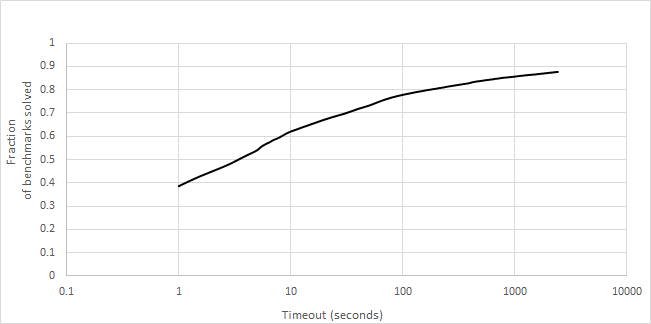
\includegraphics[width=.95\textwidth]{QF_BV-timeout-logscale2.png}
\end{center}
\caption{Solver success for QF\_BV benchmarks over time.}
\label{Fig:timeouts}
\end{figure}

There are two caveats to this observation. First, the results depend heavily on the character of the benchmarks set. Some logics have only easy benchmarks, some have purposefully crafted difficult benchmarks, others are a mix. The benchmarks are not a representative sampling of problems that might be encountered in practice.  Second, the results described are obtained by observing the wall-clock solution time when the timeout value is set at 2400 seconds. Solvers, if told what the timeout value is, have the option to adjust their search strategies based on the timeout; the solvers might then exhibit better behavior for shorter timeout.\footnote{Though solvers could use the timeout value to alter their processing algorithms, current versions of those queried\textemdash Yices2, Z3, Boolector\textemdash do not do so. However, CVC4 and CVC3 do build in the stated timeout into the script used for competition (though it is not used by the core solver) and so might show differences from the behavior stated here.}

Table~\ref{Fig:winners} shows a different view of the same data. Here we present the number of problems solved by each solver within a given wall-clock solution time, subject to the same caveats. The point to observe is that the winning solver changes depending on the timeout chosen. For these benchmarks and this set of solvers Yices2 performs best for timeouts under a second, CVC4 does best in the middle range from 1 to 200 seconds, and Boolector does best above 400 seconds. Other logics, but not all, show changes in winning order as well. This phenomenon could be a result of differences in engineering of the individual solvers or it could be a result of characteristics of the benchmark set.

The data in Table~\ref{Fig:winners} also shows that most solvers have a similar trend in success as the timeout is increased. For example, most solvers solve about 50\% (ranging from 40\% to 62\%) of the benchmarks that solver solves within the timeout by 1.0 second and
about 75\% (ranging from 65\% to 79\%) of those solved within the timeout by 10 seconds. However, some solvers, such as Boolector, are outliers: Boolector is slow off the mark - solving only 33\% and 61\% of the benchmarks it eventually solves
by 1 second and 10 seconds, respectively, even though by 2400 seconds it solves more benchmarks than any other tool, in this division.


\begin{table}
\caption{Solver success per individual solver for 2488 QF\_BV benchmarks, for different timeouts (in seconds).}
\label{Fig:winners}
\centering
\begin{tabular}{|l|rrrrrrrrrrr|}
\hline
 & \rot{4Simp} & \rot{Boolector} & \rot{CVC4} & \rot{SONOLAR} & \rot{STP-CryptoMiniSat4} & \rot{Yices2} & \rot{[CVC4-with-bugfix]} & \rot{[MathSAT]} & \rot{[Z3]} & \rot{abziz-all-features} & \rot{abziz-min-features}\\ \hline
0.5 & 824 & 683 & 886 & 712 & 728 & \textbf{963} & 830 & 608 & 919 & 839 & 840\\
1.0 & 1058 & 787 & 1089 & 928 & 923 & \textbf{1101} & 1003 & 841 & 1084 & 1043 & 1045\\
2.0 & 1184 & 979 & \textbf{1293} & 1139 & 1015 & 1187 & 1174 & 957 & 1224 & 1253 & 1252\\
4.0 & 1306 & 1158 & \textbf{1532} & 1249 & 1250 & 1261 & 1410 & 1078 & 1434 & 1444 & 1447\\
10.0 & 1581 & 1441 & \textbf{1826} & 1494 & 1433 & 1359 & 1695 & 1255 & 1620 & 1771 & 1818\\
20.0 & 1698 & 1693 & \textbf{1946} & 1563 & 1551 & 1426 & 1802 & 1424 & 1771 & 1866 & 1888\\
40.0 & 1762 & 2009 & \textbf{2155} & 1633 & 1680 & 1484 & 2017 & 1560 & 1865 & 1951 & 1961\\
100.0 & 1850 & 2150 & \textbf{2226} & 1726 & 1858 & 1563 & 2114 & 1736 & 1953 & 2091 & 2111\\
200.0 & 1912 & 2220 & \textbf{2257} & 1802 & 2025 & 1623 & 2153 & 1869 & 1997 & 2108 & 2142\\
400.0 & 1970 & 2275 & \textbf{2279} & 1892 & 2163 & 1660 & 2183 & 1999 & 2033 & 2131 & 2171\\
800.0 & 2042 & \textbf{2310} & 2296 & 1964 & 2241 & 1702 & 2222 & 2116 & 2077 & 2187 & 2223\\
1200.0 & 2074 & \textbf{2336} & 2307 & 1998 & 2256 & 1718 & 2239 & 2145 & 2106 & 2207 & 2241\\
2400.0 & 2121 & \textbf{2361} & 2307 & 2026 & 2283 & 1770 & 2239 & 2199 & 2180 & 2234 & 2277\\
\hline
\end{tabular}

\end{table}

\subsection{Application (incremental) track results}
\label{sec:application-results}

Most solvers are only concerned with raw performance on single benchmarks. However, an important application area for SMT solvers requires what the SMT-LIB standard calls `incremental' operation.
In this mode, a user or some application interacts with the solver repeatedly, issuing various commands to define a problem, check for satisfiability, inspect resulting counterexample models, adjust the problem by retracting some assertions and adding other assertions, and so on. An example use case is a tool that allows a user to author formal specifications in conjunction with software. The tool would
check using a back-end SMT solver whether the specifications are consistent with the code. If not, it might
supply a counterexample that could be inspected in conjunction with the source code. As the user edits the source or the specifications, the problem presented to the SMT solver is modified.

The application track of the competition presents to the solver a series of SMT-LIB commands through a driver program; the solver replies to the driver with a
response to each command. The driver presents commands only one at a time to emulate a realistic environment and so that the solver cannot ``work ahead.'' The driver also measures the accumulated time taken for each response. Note that the time measured includes the response time to every command, not just to the satisfiability-checking commands; while \lstinline{check-sat} commands might be the most time-consuming, \lstinline{assert} commands, and others, might also instigate significant processing. The benchmark text contains \lstinline{(set-info :status ...)} commands that
indicate the expected result for subsequent \lstinline{check-sat} commands; status information is used only by the driver program and not passed on to the solver. Such \lstinline{set-info} command might indicate a status of \lstinline{unknown}; in that case, the driver
considers the benchmark to end after the \emph{previous} \lstinline{check-sat} command for competition purposes.
The driver originally used to collect the answers had a bug that was
detected and reported by Kshitij Bansal~\cite{bansal2015email}, who
also provided a corrected version of the driver. The results discussed
in this section were obtained with this new driver and differ from those reported
earlier, such as at the 2014 SMT Workshop.

The application track was first introduced in 2011; a report on that year's application track and the overall design was presented by Griggio and Bruttomesso at the 2012 COMPARE Workshop~\cite{ag+rb+12}. A significantly adapted driver was implemented by the organizers for 2014 on the StarExec framework.

In 2014, the SMT-LIB contains 9,926 benchmarks that  specifically  exercise the incremental solving capability of solvers. Table \ref{Fig:apptrack-benchmarks} lists the numbers of benchmarks in various logics; UFLRA, QF\_UFLRA, and QF\_UFLIA are the only logics with significant numbers of benchmarks. For now, AUFNIRA does not contain any valid \lstinline{check-sat} command. All the benchmarks were used in the competition.

Four solvers participated in this competition track: CVC3, CVC4, SMTInterpol, and Yices2; Z3 was added as a demonstration-only historical comparison. The winner is the solver that solved the most \lstinline{check-sat} commands correctly within the timeout period. No solver produced an erroneous result. The time out (40 minutes) is applied to the entire benchmark, not to individual commands. The track was run for 8 divisions; the results are shown in Table \ref{Fig:apptrack-results}. Within each division, solvers are listed in winning order: Yices2 won four of the eight divisions, out of six in which it participated. CVC3, CVC4 and SMTInterpol won one division each. Since the previous execution of the application track was in 2012 and not on StarExec, we did not attempt a comparison with previous results.

\begin{table}[H]
\caption{Numbers of application benchmarks and distribution of \lstinline{check-sat} commands for different logics.}
\label{Fig:apptrack-benchmarks}
\centering
\begin{tabular}{|l|r|rrrr|}
\multicolumn{6}{c}{\textbf{All benchmarks}} \\
\hline
&  & \multicolumn{4}{c|}{{\small\bfseries\sffamily check--sat} commands} \\
 Logic & Benchmarks & total & min & max & avg. \\
\hline
AUFNIRA & 165  & 3452 & 2 & 615 & 20.9 \\
QF\_AUFLIA & 72 & 4699864 & 5 & 1109912 & 65275.9 \\
QF\_BV & 18 & 2727 & 101 & 202 & 151.5 \\
QF\_LIA & 65 & 19690826 & 101 & 2630828 & 302935.8 \\
QF\_LRA & 10 & 1515 & 101 & 202 & 151.5 \\
QF\_UFLIA & 905 & 790630 & 1 & 474174 & 873.6 \\
QF\_UFLRA & 3333 & 22103 & 2 & 3384 & 6.6 \\
UFLRA & 5358 & 3514613 & 2 & 40758 & 656.0 \\
\hline
\multicolumn{6}{c}{}\\
\multicolumn{6}{c}{\textbf{Eligible benchmarks}} \\
\hline
&  & \multicolumn{4}{c|}{{\small\bfseries\sffamily check--sat} commands} \\
 Logic & Benchmarks & total & min & max & avg. \\
\hline
AUFNIRA & 165  & 0 & 0 & 0 & 0 \\
QF\_AUFLIA & 72 & 4699864 & 5 & 1109912 & 65275.9 \\
QF\_BV & 18 & 2141 & 52 & 202 & 118.9 \\
QF\_LIA & 65 & 19689957 & 30 & 2630828 & 302922.4 \\
QF\_LRA & 10 & 795 & 45 & 107 & 79.5 \\
QF\_UFLIA & 905 & 766079 & 1 & 474174 & 846.5 \\
QF\_UFLRA & 3333 & 22066 & 0 & 3384 & 6.6 \\
UFLRA & 5358 & 223820 & 2 & 201 & 41.8 \\
\hline
\end{tabular}
\end{table}

\begin{table}
\caption{Results of the incremental track, across eight divisions. In each division, solvers are listed in winning order.}
\label{Fig:apptrack-results}
\vspace{-\medskipamount}
\centering
\resizebox{!}{294pt}{\begin{tabular}{|p{.1in}l|rrr|}
\hline
 & Solver & Commands & Wall time & CPU time \\
\hline
\multicolumn{5}{|l|}{QF\_BV (18 benchmarks, 2141 commands)} \\
& \textbf{Yices} & 1397 & 33712.3 & 33717.1 \\
& [MathSAT] & 1171 & 27308.7 & 27311.7 \\
& CVC4 & 831 & 36146.2 & 36150.9 \\
& [Z3] & 254 & 38818.0 & 38819.2 \\
\hline
\multicolumn{5}{|l|}{AUFNIRA (165 benchmarks, 0 commands)} \\
& \textbf{CVC4} & 0 & 3.0 & 0.34 \\
& [Z3] & 0 & 3.5 & 0.75 \\
& CVC3 & 0 & 3.4 & 0.52 \\
\hline
\multicolumn{5}{|l|}{QF\_AUFLIA (72 benchmarks, 4699864 commands)} \\
& \textbf{Yices} & 3244375 & 2182.6 & 2192.2 \\
& [Z3] & 3244375 & 8564.3 & 8335.6 \\
& SMTInterpol & 3244375 & 9442.9 & 9703.8 \\
& CVC4 & 114063 & 38840.4 & 38835.8 \\
& [MathSAT] & 377 & 115201.7 & 115200.5 \\
\hline
\multicolumn{5}{|l|}{QF\_LIA (65 benchmarks, 19689957 commands)} \\
& \textbf{Yices} & 19689907 & 36664.0 & 36745.5 \\
& [Z3] & 19688439 & 58239.0 & 57902.7 \\
& SMTInterpol & 19687199 & 72449.4 & 73946.1 \\
& [MathSAT] & 15214533 & 58005.2 & 57747.8 \\
& CVC4 & 4265295 & 97269.3 & 97410.6 \\
\hline
\multicolumn{5}{|l|}{QF\_LRA (10 benchmarks, 795 commands)} \\
& \textbf{Yices} & 742 & 9592.5 & 9536.6 \\
& [MathSAT] & 688 & 7569.4 & 7571.7 \\
& SMTInterpol & 445 & 12104.9 & 12295.4 \\
& [Z3] & 410 & 17398.3 & 17400.1 \\
& CVC4 & 222 & 19521.0 & 19522.0 \\
\hline
\multicolumn{5}{|l|}{QF\_UFLIA (905 benchmrks, 766079 commands)} \\
& [Z3] & 766050 & 35438.9 & 35422.1 \\
& \textbf{Yices} & 762593 & 432909.7 & 432549.4 \\
& CVC4 & 762579 & 175681.8 & 173808.4 \\
& SMTInterpol & 761675 & 202682.2 & 208723.0 \\
& [MathSAT] & 757329 & 256114.4 & 255888.5 \\
\hline
\multicolumn{5}{|l|}{QF\_UFLRA (3333 benchmarks, 22066 commands)} \\
& \textbf{Yices} & 22053 & 55654.4 & 55151.1 \\
& [Z3] & 22043 & 37848.1 & 37596.8 \\
& SMTInterpol & 21658 & 120249.0 & 130229.8 \\
& [MathSAT] & 21514 & 35899.4 & 35711.5 \\
& CVC4 & 20295 & 104716.5 & 103715.5 \\
\hline
\multicolumn{5}{|l|}{UFLRA (5358 benchmarks, 223820 commands)} \\
& [Z3] & 222579 & 370913.4 & 368869.9 \\
& \textbf{CVC3} & 67802 & 194697.8 & 192840.6 \\
& CVC4 & 65360 & 2816349.8 & 2802724.6 \\
\hline
\end{tabular}
}
\end{table}

We can also consider the effect of the choice of timeout on the application track. This effect is more complicated than for the main track since an application track benchmark can have partial results. For example, if a benchmark contains 100 check-sat commands, a solver may report correct answers on 0 to 100 of them prior to timing out. Furthermore the seven divisions that have results show very different characteristics. In four of the divisions (QF\_AUFLIA, QF\_UFLIA, QF\_UFLRA, UFLRA) over 90\% of the solver-benchmarks jobs were completed before the timeout; for QF\_UFLRA it was over 99\%. The other three divisions (QF\_BV, QF\_LIA, QF\_LRA) had much harder benchmarks. For example, for QF\_BV, only 1\% of solver-benchmark pairs were completely solved by 1 second and only 42\% by the timeout.  These three divisions also have many fewer benchmarks---a few hundred, rather than several thousand. Changing the timeouts further might affect the results of these divisions significantly, but not those of the four divisions with many more benchmarks.

\section{FLoC Olympic Games Scoring}
\label{sec:floc}

The main track and the application track described in previous sections are staples of recent SMT Competitions. The 2014 edition was unique in also being associated with the FLoC Olympic Games~\cite{FLoCGames}.
This association was positive in providing a platform, along with the other competitions, to present the
rationale, methodology and results of the SMT Competition to a wider audience than just the SMT community.

One additional aspect that resulted from the Olympic Games was the awarding of three medals to the three ``winners'' of the competition. Since SMT-COMP is organized into many separate divisions, with winners determined in each division independently, the organizers had to determine how to award three global prizes.
The metrics for doing so were the subject of significant discussion both before and after the competition.
The metrics were decided by the organizers before the competition began (and before the deadline for solver registration) and were maintained unchanged after the competition.

The organizers chose to award the bronze medal for the best performance in a single division. We chose  the QF\_BV division for this medal because it is significant to applications and because it traditionally received the most solver submissions. Indeed in 2014, there were 8 participants. Determining the winner was straightforward: we used the same metric as is used for each division\textemdash the most problems solved without errors, with ties broken by speed of solution. The Boolector~\cite{boolector} solver won this division and therefore the bronze medal. The results for all participating solvers are shown in Table \ref{Table:bronze}.

The organizers chose to award the silver and gold medals for best performance across the most divisions. Thus we needed a metric that combined the results across divisions. We considered two metrics. For a given solver, let
\begin{itemize}[noitemsep,nolistsep]
\item $e_i$ be the number of benchmarks in division $i$ for which an incorrect result was produced (that excludes timeouts, runtime errors and \lstinline{unknown} answers);
\item $c_i$ be the number of benchmarks in division $i$ solved correctly;
\item $t_i$ be the total time to solve the benchmarks in division $i$ that were solved correctly;
\item $N_i$ be the total number of benchmarks in division $i$, used in the competition.
\end{itemize}
The normal metric for a division is that the winning solver is the one with the
smallest value of $e_i$, the largest value of $c_i$
and then the smallest value of $t_i$, for each division taken separately;
that is, the metric is a lexicographic ordering by smallest value of $\langle e_i, -c_i, t_i \rangle$.
The two global metrics we considered are
\begin{itemize}[noitemsep,nolistsep]
\item Metric A: The winning solver is the one with the smallest value of $\sum_i e_i \log N_i$, then the largest value of $\sum_i (c_i/N_i)^2 \log N_i$, then the smallest value of $\sum_i t_i \log N_i$, where for a given solver the sums are over all competitive divisions in which that solver participated.
\item Metric B: The winning solver is the one with the largest value of $\sum_i (e_i == 0\,?\,(c_i/N_i)^2 : - e_i ) \log N_i$, then the smallest value of $\sum_i t_i \log N_i$, where for a given solver the sums are over all competitive divisions in which that solver participated.
\end{itemize}

Note that incorrect results are very rare in SMT-COMP, but do occur; for almost all solvers and divisions the value of $e_i$ is 0 and the competition hinges on the values of $c_i$. The speed of the solver is important in two ways. First, if the solver is slow, it will time out before a solution is found and thus the value of $c_i$ will be lower. Second, if there is a tie in the number of errors and correctly solved problems, the total time taken on the correctly solved problems is used as the tie-breaker (even if the solvers solve different subsets of benchmarks); this is a rare occurrence but does happen if, for example, all the benchmark problems in a division are solvable within the time limit---the only situation in the competition in which tie-breaking has been needed. 

Only \emph{competitive divisions} were included in the scoring (although all divisions were run and results reported). For determining medals, a division is competitive if there are at least two officially registered, participating solvers \emph{from different teams}. This prevents a team from gaming the scoring by submitting multiple solvers to divisions in which no one else is participating. This criterion excluded a number of divisions from medal scoring: AUFNIRA, BV, NIA, NRA, QF\_UFNIA, QF\_UFNRA, UFBV, UFIDL, UFNIA.

The log scaling of the scores for each division is a somewhat arbitrary means to adjust the scores for the wide variety of numbers of benchmarks. If each division is treated equally, with a score, say, of 1.0 for the division for solving all the benchmarks in the division correctly, then the benchmarks for small divisions would count significantly more toward a composite score than those of divisions with many benchmarks. On the other hand, counting each benchmark equally appeared to underweight the effect of a solver's effort to participate in multiple divisions. The log scaling seemed a reasonable compromise between these two extremes. Similarly, the square of the fraction successfully solved is an approximate mechanism to give more weight to solving the harder problems.

Metrics A and B above differ in how errors are treated. If a solver has no errors, it is always better off to participate in as many divisions as possible. However, an error in a division penalizes a solver so that it would be better not to have participated in the division; hence the organizers ruled that once the competition had started, a solver could not be withdrawn from a division in which it was registered.

The penalty for an error is globally significant in Metric A: a single error in one division out of many would put the solver behind any other solver with no errors, even if that other solver participated in just one division. The penalty for an error is more local for Metric~B: the error results in a large negative score for that division, which might be compensated by good performance in other divisions. Both metrics satisfy the criterion of putting heavy weight on correctness of solvers.
The organizers published the choice of Metric A as the metric for the Olympic Games gold and silver medals in the rules prior to the beginning of the competition, with no objection during the comment period. 

Though all solvers were scored for the medal metrics, five solvers participated in more than two divisions and were the most competitive during the course of the competition. The final results are shown in Table \ref{Table:medals}. The choice of metric did have a significant effect on the result. CVC4 and Yices2 participated in the most divisions, solved the most problems, and did so the most efficiently. However, Yices2 had a crash on one problem in QF\_ABV, but had emitted an erroneous answer prior to the crash (a simple crash without an answer is scored the same as an `unknown' response, marked neither wrong nor correct). CVC4 had bugs that affected AUFNIRA, which was not a competitive division, and QF\_LIA,
which was competitive. Consequently, by the competition metric, these two otherwise leading solvers placed much further back in the pack.

When the results were published, the resulting winning teams, veriT and SMTInterpol, put an appeal to the organizers to use Metric B instead, arguing that (i)~CVC4 and Yices2 were clearly the more capable solvers and (ii)~there were known bugs in the winning solvers as well, which, simply by good fortune, were not triggered by the competition benchmarks. However, after public comment acknowledging the good will of the winners, the appeal was not accepted by the organizers. The medal ceremony did highlight the differing contributions of all four teams as well as those of the bronze medal winner. Note that the discovered bugs were promptly fixed. In fact, CVC4 submitted an additional demonstration-only version, named CVC4-with-bugfix in the result tables, which the organizers ran in conjunction with the rest of the competition.

\begin{table}
\caption{Gold and silver medal competition, in winning order by Metric A. By Metric B the order is the same except that CVC4 and Yices2 are in first and second place.}
\label{Table:medals}
\centering
\begin{tabular}{|l|r|rr|r|}
\hline
Solver  & Competitive & Metric A & & Metric B \\
 & Divisions & Weighted errors & Weighted solved & \\
\hline
veriT & 17 &	0.000 	& 	25.325 & 25.325 \\
SMTInterpol & 8 &	0.000 	& 	22.831 & 22.831 \\
CVC3 & 10	& 	0.000 	& 	9.618 & 9.618 \\
SONOLAR 	& 2	&  	0.000 	& 	5.978 & 	5.978\\
AProVE 		& 1 & 	0.000 	& 	3.776	& 	3.776\\
Boolector-j & 1	&  	0.000 	& 	3.758	& 	3.758\\
Boolector-d & 1		&  	0.000 	& 	3.755 & 	3.755\\
OpenSMT2 	& 1	&  	0.000 &	3.582 &	3.582\\
Boolector & 1		&  	0.000 &	3.058  &	3.058 \\
STP-CryptoMiniSat4 	& 1	&  	0.000 &	2.859 &	2.859\\
4Simp 	& 1	& 	0.000 	& 	2.468  	& 	2.468 \\
raSAT 	& 1	& 	0.000 	& 	0.000 	& 	0.000 \\
Yices2 	& 15	&  	3.810 	& 	38.624 & 31.059 \\
CVC4 		& 25 &  	7.283 	& 	54.152 & 43.509 \\
abziz\_min\_features 	& 1	& 	30.563 	& 	2.548 & -30.563 \\
abziz\_all\_features 	& 1	&  	30.563 	& 	2.403 & -30.563 \\
Kleaver-STP 	& 1	&  	213.362 	& 	3.103 & -213.362 \\
Kleaver-portfolio & 1		&  	346.713 	& 	3.073  & -346.713 \\
\hline
\end{tabular}
\end{table}

\begin{table}
\caption{Bronze medal competition (QF\_BV division, 2488 benchmarks), in winning order.}
\label{Table:bronze}
\centering
\begin{tabular}{|l|rrr|}
\hline
 Solver & Errors & Solved & Time (sec)\\
\hline
Boolector &	0  &		2361  &		138077.59 \\
STP-CryptoMiniSat4 & 0  &		2283  &		190660.82 	\\
{[}CVC4-with-bugfix] &	0  &		2237 	 &		139205.24 \\
{[}MathSAT]  &	0  &		2199 	 &		262349.39 \\
{[}Z3]  & 	0  &		2180 	 &		214087.66 	\\
CVC4  &	0  &		2166 	 &		87954.62 	\\
4Simp &	0 &	2121 	 &		187966.86 \\
SONOLAR &	0  &		2026  &	 	174134.49 \\
Yices2 &	0  &		1770  &	 	159991.55 \\
abziz\_min\_features &	9  &		2155 	 &	 	134385.22 \\
abziz\_all\_features &	9  &		2093 	 &	 	122540.04 \\
\hline
\end{tabular}
\end{table}

\section{Post-Competition Activity}
\label{sec:post}

After the competition, David Cok (competition chair) and Clark Barrett and Morgan Deters (SMT-LIB coordinators) collaborated, with the assistance of Aaron Stump (StarExec lead), in attempting to discover the status of the SMT-LIB benchmarks that were marked as unknown. For this computation, the timeout was set to 10 hours. This activity required several weeks of computation. A result confirmed by at least two solvers was obtained for 75\% of the unknown benchmarks, with another 4\% having a tentative result from just one solver.
The results are shown in Table~\ref{Fig:post}.

The unknown incremental benchmarks have yet to be resolved.

\begin{table}
\caption{Benchmarks resolved in post-competition computation}
\label{Fig:post}
\centering
\begin{tabular}{|l|c|r|rr|rr|r|}
\hline
Logic & Solvers & {\pbox{1.1in}{Unknown\\Benchmarks}} & \multicolumn{2}{c|}{\pbox{1.1in}{Resolved by\\2+ solvers as}} & \multicolumn{2}{c|}{\pbox{1.1in}{Resolved by \\ 1 solver as}} & \pbox{.6in}{Still\\unknown} \\
 & & & sat & unsat & sat & unsat & \\
\hline
AUFLIRA & 2 & 168 & 0 & 3 & 0 & 3 & 162 \\
AUFNIRA & 2 & 468 & 0 & 23 & 0 & 23 & 422 \\
BV & 2 & 191 & 29 & 56 & 42 & 37 & 27 \\
LRA & 2 & 450 & 20 & 148 & 241 & 23 & 18 \\
NRA & 2 & 66 & 0 & 41 & 0 & 16 & 9 \\
QF\_ABV & 4 & 4190 & 3629 & 373 & 0 & 1 & 187 \\
QF\_BV & 4 & 28138 & 8838 & 19166 & 20 & 10 & 100 \\
QF\_IDL & 3 & 537 & 324 & 118 & 20 & 14 & 61 \\
QF\_LIA & 3 & 1279 & 743 & 230 & 234 & 4 & 68 \\
QF\_LRA & 2 & 208 & 127 & 25 & 44 & 8 & 4 \\
QF\_NIA & 3 & 927 & 2 & 0 & 39 & 246 & 640 \\
QF\_NRA & 2 & 1392 & 0 & 36 & 283 & 168 & 905 \\
QF\_RDL & 2 & 85 & 50 & 0 & 2 & 1 & 32 \\
QF\_UF & 3 & 4 & 0 & 3 & 0 & 1 & 0 \\
QF\_UFLRA & 3 & 87 & 82 & 2 & 2 & 0 & 1 \\
QF\_UFNRA & 2 & 11 & 0 & 2 & 7 & 0 & 2 \\
UF & 2 & 2911 & 0 & 2 & 51 & 50 & 2808 \\
UFBV & 2 & 191 & 17 & 49 & 51 & 44 & 30 \\
UFIDL & 2 & 12 & 0 & 0 & 0 & 0 & 12 \\
UFLIA & 2 & 5499 & 0 & 1765 & 4 & 113 & 3617 \\
UFNIA & 2 & 1052 & 0 & 20 & 2 & 90 & 940 \\
\hline
Total & & 47866 & 13861 & 22062 & 1042 & 852 & 10045 \\
\hline
\end{tabular}
\end{table}

\section{Concluding Observations and Recommendations}
\label{sec:conclusions}

SMT-COMP 2014 successfully executed the comparison among solvers that is the main goal of the competition. The new computational infrastructure, StarExec, worked very well for the purpose. The competition saw a renewed interest in participation\textemdash there were record numbers of teams participating, solvers entered, teams and solvers that had never before participated, benchmarks used, and amount of computation performed. Although the 2014 results are not readily comparable to previous years (because of changes in benchmarks and equipment), the detailed performance of each solver on each benchmark from this first year using StarExec will be a solid baseline to measure improvements in the state-of-the-art of solver performance in future years. As a partial comparison, solvers that performed well in previous years were included in this year's competition.

The SMT steering committee proposed that SMT-COMP 2015 be held in association with the SMT Workshop, which itself will be affiliated with CAV 2015 in San Franciso, CA, USA from July 18-24, 2015.  The SMT Workshop is being organized by Vijay Ganesh and Dejan Jovanovi\'c; the organizers of the competition are Tjark Weber, David D\'eharbe, and Sylvain Conchon.

\paragraph{Observations}

Solver implementors continue to focus primarily on raw numbers of problems solved. We think that future competitions can 
help broaden the focus to encompass breadth of problems addressed, fast solutions on simple problems, and other features provided by the SMT-LIB command language.

An unexpected observation is that there is indeed a difference in outcome of even a straightforward competition depending on the value of timeout chosen. As a result, there might indeed be an interest and valuable result from trying a competition track focused on fast solving of relatively simple problems.

A satisfying observation is that there is reasonable competition among several highly-performing solvers, as measured by the unique contributions each makes and the distribution of fastest times.

\paragraph{Recommendations.} Based on the experience of 2014, the 2014 organizers have the following recommendations or topics for consideration for future competitions.
\begin{itemize}
\item The 2014 competition used all available benchmarks; though the computation resources enable using all benchmarks, future competitions should consider how to make a principled selection to avoid over-representing benchmarks of particular types or origin.
\item The competition has used numbers of solved benchmarks as the primary success criterion. Time to solve benchmarks should be considered more strongly. In particular, a separate track that emphasizes fast solution of fairly simple problems might be informative.
\item Related to the previous point, currently if a solver times-out or issues a response of `unknown', the time taken to do so is not counted in the accumulated time. Only the time taken to compute correct responses is counted towards the evaluation metric.
A user's experience, however, is that the time taken for a solver to say ``I don't know'' is just as important as time to produce a useful answer. Thus we recommend that such
computation time be included in the evaluation metric. Omitting this time has had no effect so far because time was little used in the overall metric.
\item The comparison to a previous years' results will now be easier because common hardware will be used and benchmark selection is simplified. Future organizers might also include a larger selection of the specific solver versions that were entered in previous competitions. 
\item A key improvement needed is better benchmark sets. Though the accumulation of benchmark problems since the inception of the competition is impressive, attention now needs to be paid to the quality and distribution of benchmarks. Some divisions are represented by only a few benchmarks; others have large numbers of similar benchmarks.
Benchmarks representative of application scenarios are particularly important.
\item Subsequent to SMT-COMP 2014, David Cok, Aaron Stump, Morgan Deters, and Clark Barrett collaborated in resolving the status of many previously unknown benchmarks. Those new expected results are not yet included in the SMT-LIB benchmarks on StarExec. They should be incorporated into SMT-LIB on StarExec prior to the next competition.
\item If a global metric is needed again in the future (per \S\ref{sec:floc}), a review and re-discussion of the appropriate metric should be instigated.
\item Solvers with breadth of application across many logics and solvers that address problems in new logics such as string and floating point computations are important to users. Future competitions should add tracks or otherwise find means to reward solvers that implement such capabilities.
\item Various competition tracks used in the past should be rejuvenated: parallel processing, computation of unsat cores, production of proofs, computation of symbolic models, and computation of concrete counterexamples.
\item One missing tool is a standard SMT-LIB syntax checker. jSMTLIB~\cite{cok2011jsmtlib} has been proposed for this purpose, but is not yet integrated into StarExec. The tool also needs to be updated to include the proposed new SMT-LIB features.
\item The difficulty in preparing a new solver for submission to StarExec for participation in SMT-COMP should be reduced.
\item A general means to resolve questions surrounding partial definitions is needed in SMT-LIB, e.g., for divide-by-zero  (cf.~\S\ref{par:undefined}).
\item An item for study is the effect of benchmark scrambling on the outcome of solver comparisons.
\item Clearly define the subset of SMT-LIB~v2 that solvers must support for a competition and that benchmarks must use.
\end{itemize}

\section*{Acknowledgments}

\begin{itemize}
\item The organizers were supported by their respective institutions (GrammaTech, Federal University of Rio Grande do Norte, Brazil and Uppsala University, Sweden respectively).  In addition, Cok received partial support from the U.S.\ National Science Foundation under grant ACI-1314674.

\item Clark Barrett and Morgan Deters assisted with some aspects of benchmark preparation, in their roles as SMT-LIB coordinators.

\item Aaron Stump and the StarExec support team were essential in keeping the competition cluster running; in this first large-scale, public use of the cluster, numerous small details needed correction and were corrected promptly.  The StarExec cluster is supported by the U.S.\ National Science Foundation under grants \#1058748 and \#1058925.
  
\item The cost of executing the SMT Competition is underwritten by the SMT Workshop.
\end{itemize}

Any opinions, findings, and conclusions or recommendations expressed in this material are those of the authors, and do not necessarily reflect the views of the National Science Foundation.

\bibliographystyle{plainbv}
\bibliography{SMTCOMP}

\end{document}

%% Local Variables:
%% mode: LaTeX
%% ispell-local-dictionary: "american"
%% mode: flyspell
%% LocalWords: Tjark Uppsala
%% End:
